%!TEX program = <xelatex>
\documentclass[12pt,letterpaper]{article}

\usepackage{basicstyle}
\usepackage{notestyle}

\title{Notes on CS6363}
\author{Hanlin He}
\date{\today}

\makeindex
\begin{document}

\maketitle

\pagebreak

\pagenumbering{Roman}
\tableofcontents
\pagebreak
\listofalgorithms
\pagebreak

\pagenumbering{arabic}

\section{Syllabus}
\begin{enumerate}
\item Asymptotic  notation, recurrence.
\item Divide and Conquer.
\item Dynamic Programming.
\item Greedy Algorithm.
\item Graph Algorithm.
\item NPC
\end{enumerate}


\pagebreak

\section{Basic}
\subsection{What is an algorithm?}
Unambiguous, mechanically executable sequence of elementary operations.

There are certain types of algorithm:

\begin{tabular}{ ll }
Traditional (This course’s main focus.) & Modern algorithm research\\
\hline
Deterministic & Randomized \\
Exact & Approximate\\
Off-line & On-line\\
Sequential & Parallel\\
\end{tabular}

\subsection{Input \& Output}

View algorithm as a function with well defined inputs mapping to specific
outputs. For example:

\begin{quote}

\AlgoInput $A[1...n]$  // Positive real number, distinct.

\AlgoOutput $MAX A[i], 1<= i <= n$.

\end{quote}

\subsubsection{Algorithm 1}

Stupid way.

\begin{algorithm}[H]
\caption{Stupid Find Max Algorithm}\label{Stupid_Find_Max_Algorithm}
\begin{algorithmic}[1]
\Procedure{FindMax}{}
\For{$i = 1$ to $n$}
  \State $count = 0$
  \For{$j = 1$ to $n$}
    \If{$A[i] > A[j]$}
      \State $count = count + 1$
    \EndIf
  \EndFor
  \If{$count = n$}
    \State \textbf{return} {$A[i]$}
  \EndIf
\EndFor
\EndProcedure
\end{algorithmic}
\end{algorithm}

\textbf{Analysis}: Worst Case, $n^2$ comparison.

\subsubsection{Algorithm 2}

Sort \& Find.

\begin{algorithm}[H]
\caption{Sort \& Find Max Algorithm}\label{Sort_and_Find_Max_Algorithm}
\begin{algorithmic}[1]
\Procedure{FindMax}{}
\State {$\overline{A} = sort(A)$}
\State \textbf{return} {$\overline{A}[n]$}
\EndProcedure
\end{algorithmic}
\end{algorithm}

\textbf{Analysis}: Worst Case, sorting takes $c\ n\log n$ time.

\subsubsection{Algorithm 3}

Dynamically store the biggest one.

\begin{algorithm}[H]
\caption{Search \& Find Max Algorithm}\label{Search_and_Find_Max_Algorithm}
\begin{algorithmic}[1]
\Procedure{FindMax}{}
\State {$current = 1$}
\For{$i = 2$ to $n$}
  \If{$A[i] > A[current]$}
    \State{$current = i$}
  \EndIf
\EndFor
\State \textbf{return} {$A[current]$}
\EndProcedure
\end{algorithmic}
\end{algorithm}

\subsection{Can we do better?}

It depends on the operations allowed. For example the dropping the curtain and
find the first appearing one.


\pagebreak


\section{Asymptotic Notation -- big ``O'' notation}

\subsection{Growth of Functions}

The growth of function in \cref{function_list} increase downwards.
\begin{table}[H]
\centering
\caption{Function List}\label{function_list}
\begin{tabular}{c|l}
$\log_{10} n$ & binary search \\
$n$ & input \\
$n^2$ & pairs \\
$10^{10}n^{10}$ & \\
$1.000.1^n$ & \\
$2^n$ & Binary string of length n \\
$n!$ & Permutation \\
\end{tabular}
\end{table}
Let $f(n)$, $g(n)$ be function.

\subsection{big ``O'' notation}
\begin{definition}

$f(n) = \bigO{g(n)}$, if $\exists n_0 \in \mathbb{N}$,
$c \in \mathbb{R}^+$, s.t. $\forall n \geq n_0$, $f(n) \leq c * g(n)$,
and $\lim_{n \rightarrow \infty} \frac{f(n)}{g(n)} \ne \infty$, i.e.\ it is $\lim_{n \rightarrow \infty} \frac{f(n)}{g(n)} < k$, for some constant $k$.
\end{definition}

Table \ref{def_asymptotic_notation} shows the basic definition of all the asymptotic notations.
\begin{table}[H]
\centering
\caption{Definition for all Asymptotic Notation}\label{def_asymptotic_notation}
\begin{tabular}{c|l|c}
\hline
$f(n)$ & $\lim_{n \rightarrow \infty} \frac{f(n)}{g(n)}$ & relation \\
\hline
\hline
$\bigO{g(n)}$ & $\neq \infty$ & $\leq$ \\
$\Omega(g(n))$  & $\neq \infty$ & $\leq$  \\
$\Theta(g(n))$  & $= k > 0$ & $=$  \\
$o(g(n))$  & $= 0$ & $<$  \\
$\omega(g(n))$  & $= \infty$ & $>$  \\
\end{tabular}
\end{table}

\subsection{Asymptotic Relation's feature}
\begin{theorem}
Multiplying by positive constant does NOT change asymptotic relations.
i.e.\ if $f(n) = \bigO{g(n)}$, then $100 * f(n) = \bigO{g(n)}$.
\end{theorem}

\begin{proof}
$f(n) = \bigO{g(n)} \Rightarrow \exists{n_0} \exists c, \forall n \geq n_0, f(n) \leq c*g(n)$,

then, $\exists{n_0}\exists{c'}$, s.t.\ $\forall n \geq n_0$, $100*f(n) \leq c'*g(n) = 100c*g(n)$.
\end{proof}

Example:
\begin{align}
C*2^n & = \Theta(2^n) \\
(C*2)^n & \neq \Theta(2^n)
\end{align}

\begin{claim}
Show: $2n\log(n) - 10n = \Theta(n\log(n))$
\end{claim}

\begin{proof}
First show: $2n\log(n) - 10n = \bigO{n\log(n)}$

For $n_0 = 1$, $c = 2$

\[2n\log(n) - 10n \leq 2n\log(n)\]

Now show: $2n\log(n) - 10n = \Omega(n\log(n))$

For $n_0 = 2^10$, $c = 1$,

\[
\begin{split}
2n\log(n) - 10n & \geq n\log(n) + n \log(2^{10}) - 10n \\
& =n \log(n) + 10n - 10n \\
& =n\log(n) \\
\end{split}
\]

$n_0 = 1$ ($n_0 = 2^{10}$) means $n$ is at least $1$ (or $2^{10}$).
\end{proof}

\begin{corollary}
$\bigO{1}$ means \textbf{Any Constant}.
\end{corollary}

\textbf{Attention}: \emph{Asymptotic notation has limit. It is not applicable for all scenarios}.

\subsection{Properties of \texorpdfstring{$\log(n)$}{log(n)}}
\definition{$n = C^{\log_c{n}}$, $c > 1$, $\lg{n} = \log_2{n}$, $\ln{n} = \log_e{n}$.}

\begin{corollary}
$\forall{a,b} > 1$

\begin{equation}
\begin{split}
\log_b(n) & = \frac{\log_a(n)}{\log_a(b)} \\
\log_b(n) & = \Theta({\log_a(n)}) \\
\end{split}
\end{equation}

\end{corollary}

\begin{corollary}
$\forall{a,b} \in \mathbb{R}$

\begin{equation}
\begin{split}
\log(a^n) & = n*\log(a) \\
\log(a*b) & = \log(a) + \log(b)) \\
a^{\log(b)} & = b^{\log(a)} \\
\end{split}
\end{equation}

\end{corollary}

\textup{\textbf{Note}: $\lg(n)$ is to $n$ as n is to $2^n$.}

\subsection{Something More}

\begin{theorem}
Let $f(n)$ be a polynomial function, then $\log(f(n)) = \Theta(\log(n))$.
\end{theorem}

\begin{proof}
The asymptotic result of $n^2$ and $n^10$ are the same.
\end{proof}

\begin{definition}
$\log^*(n) = o(\log\log\log\log\log(n)) = \alpha$.
\end{definition}

Example: $\lg^*(2^{2^{2^{2^{2}}}}) = 5$.


\pagebreak


\section{Series}
\subsection{Some Definition}

\begin{definition}
Harmonic Series:
\[\sum_{i=1}^n {\frac{1}{i}} = \Theta(\log(n))\]
\end{definition}

\begin{definition}
Geometric Series:
\[
\sum_{i=0}^{n-1}{x^i} = \frac{x^n - 1}{x-1} =
\begin{cases}
\Theta(x^n) & \text{if } \forall x>1, \\
\Theta(1) & \text{if } \forall x<1, \\
\Theta(n) & \text{if } \forall x=1.
\end{cases}
\]
\end{definition}

\begin{definition}

Arithmetic Series:

\[\sum_{i=1}^n {i} = \frac{n(n+1)}{2} = \Theta(n^2)\]

\end{definition}

\subsection{Some Theorem}

Suppose I want to know if $f(n) = o(g(n))$.

\begin{theorem}
If $\log(f(n)) = o(\log(g(n))$, then $f(n) = o(g(n))$.
\end{theorem}

Example: Let $f(n) = n^3$, $g(n) = 2^n$. Then $\log(f(n)) = \log(n^3) = 3\log(n)$, $\log(g(n)) = \log(2^n) = n$.
\[\text{i.e. } \log(f(n)) < \log(g(n) \Rightarrow f(n) < g(n)\]

\emph{Note that this theorem stands for `o', NOT TRUE for `$\mathcal{O}$'.}

Example: $\log(n^3) = \mathcal{O}(\log(n^2))$, but $n^3 \neq \mathcal{O}(n^2)$.

\section{Induction}
\subsection{When to use?}

Prove statement for all $n \in \mathbb{N}$, s.t. $n \geq n_0$.

\subsection{Definition}
Basically, induction has two parts:
\begin{enumerate}
\item {Base case(s) -- Sometimes there are more than one base cases.

Prove statement for some $n$. -- Often $n_0 = 0 \text{ or } 1$.}

\item {Induction Hypothesis

Assume statement hold true for all $m \leq n$.

Prove the hypothesis implies that it hold true for $n+1$.}
\end{enumerate}

Note that the process may be different from previous, which just hypothesize $n-1$ is true and prove for $n$.

\subsection{Example}
\subsubsection{Good Induction:}

\Claim  $\displaystyle\sum _{i=1}^n i = \frac{n(n+1)}{2}$

\begin{proof}
We are required to prove $\displaystyle\forall n > 0 \text{, } \sum _{i=1}^n i = \frac{n(n+1)}{2}$.


\BaseCase $n=1$, $\displaystyle\sum _{i=1}^1 i = 1 = \frac{1\times (1+1)}{2}$. Hence the claim holds true for $n=1$.

\InductionStep Let $k > 1$ be an arbitrary natural number.

Let us assume the induction hypothesis: for every $k < n$, assume $\displaystyle\sum _{i=1}^k i = \frac{k(k+1)}{2}$. We will prove $\displaystyle\sum _{i=1}^{k+1} i = \frac{(k+1)(k+2)}{2}$

\begin{equation}
\sum _{i=1}^{k+1} i = \left(\sum _{i=1}^{k} i \right) + (n+1)
                    = \frac{k(k+1)}{2} + \frac{2(k+1)}{2}
                    = \frac{(k+1)(k+2)}{2}
\end{equation}

Thus establishes the claim for $k+1$.

\InductionConclusion By the principle of mathematical induction, the claim holds for all $n$.
\end{proof}

\subsubsection{Bad Induction: Prove all horses are the same color}

The process is omitted. The key point is that: if the base case is not true for induction hypothesis, the induction will not be solid.






\pagebreak

\section{Recursion (Divide \& Conquer)}
\begin{itemize}
\item Recursion is like Induction's twin brother, whereas induction is similar to movie filmed, and recursion is similar to movie backward.
\item Recursion design may be most important course topic.
\item Recursion is a type of reduction. \footnote{Reduction is to solve problem A using a black box for B. Typically B is smaller.}
\end{itemize}

\subsection{Definition of Recursion: a Powerful type of reduction}
\begin{enumerate}
\item if problem size very small (think $\mathcal{O}(1)$), just solve it.
\item reduce to one or more small instances of some problem.
\end{enumerate}

\question How are the smaller (but not $\mathcal{O}(1)$ size) problem solved?

Not your problem! Handled by the recursion fairy.

\subsection{Tower of Hanoi}
\subsubsection{Description of Problem}
\begin{itemize}
    \item 3 pegs, which hold n distinct sized disks.
    \item initially $tmp$, $dst$ empty and $src$ has all disks sorted.
    \item 3 rules:
    \begin{enumerate}
        \item larger cannot be placed on smaller.
        \item only one disks can move at a time.
        \item move all disks to $dst$.
    \end{enumerate}
\end{itemize}

\question How long until the world end?

\subsubsection{Analysis}
A small hint: not consider the smallest first, but the largest first.

In order to move the largest disk:
\begin{itemize}
    \item $dst$ has to be empty.
    \item $src$ has only largest one.
    \item $tmp$ has $n-1$ disks sorted.
\end{itemize}

So we must:
\begin{enumerate}
    \item move $n-1$ disks from $src$ to $tmp$\tikzmark{hanoi1}{.}
    \item move largest from $src$ to $dst$\tikzmark{hanoi2}{.}
    \item move $n-1$ disk from $tmp$ to $dst$\tikzmark{hanoi3}{.}

    \begin{tikzpicture}[remember picture,overlay,node distance = 3cm]
        \node (hanoi12descr) [right =of hanoi2]{Don't know how to do.};
        \node (hanoi12descrdescr) [below =1cm of hanoi12descr]{\textbf{Don't think about it!!}};
        \draw[red,->,thick] (hanoi1) to [in=-180,out=0] (hanoi12descr);
        \draw[blue,->,thick] (hanoi3) to [in=-180,out=0] (hanoi12descr);
        \draw[purple,->,thick] (hanoi12descr) to [in=90,out=-90] (hanoi12descrdescr);
    \end{tikzpicture}
\end{enumerate}

Don't think about how to move $n-1$ disks, recursion fairy will do it.

\begin{algorithm}[h]
    \caption{Recursive Hanoi}\label{rec_hanoi}
    \begin{algorithmic}
        \Procedure{Hanoi}{$n, src, dst, tmp$}
            \If{$n>0$}
                \State \ProcedureName{Hanoi}{n-1, src, tmp, dst}
                \State Move disk $n$ from $src$ to $dst$.
                \State \ProcedureName{Hanoi}{n-1, tmp, dst, src}
            \EndIf
        \EndProcedure
    \end{algorithmic}
\end{algorithm}

How many moves in \cref{rec_hanoi} ?

Let $T(n)$ be the total moves for $n$ disks.
\begin{align*}
    T(0) &= 0 \\
    T(1) &= 1 \\
    T(n) &= T(n-1) + 1 + T(n-1) \\
         &= 2T(n-1) + 1
\end{align*}

``Solve'' the recurrence.
\[\sum_{l=1}^n 2^{l-1} = 2^n - 1\]

\subsection{Binary Search}

\AlgoInput Given a value $val$, and sorted aray $A[1 \ldots n]$.

\AlgoOutput Is $val$ contained in $A$?

\begin{algorithm}[H]
\caption{Binary Search Algorithm}\label{bianry_search}
\begin{algorithmic}[1]
\Procedure{Bin}{$val, low, high$}
  \If{$high < low$}
    \Return Not Found
  \EndIf
  \State $mid = \big\lfloor\frac{high + low}{2}\big\rfloor$
  \If{$val < A[mid]$}
    \Return \ProcedureName{Bin}{val, low, mid-1}
  \EndIf
  \If{$val > A[mid]$}
    \Return \ProcedureName{Bin}{val,mid+1,high}
  \EndIf
  \Return $mid$
\EndProcedure
\end{algorithmic}
\end{algorithm}

To find whether $val$ is contained in $A[1\ldots n]$, call \ProcedureName{Bin}{val,1,n}.

Let $m = high - low + 1$,

\begin{align}
T(m) & \leq \max\bigg\{T\Big(\Big\lfloor\frac{m-1}{2}\Big\rfloor\Big)\tikzmark{floorceil},
                       T\Big(\Big\lceil\frac{m-1}{2}\Big\rceil\Big)\bigg\}
                       + \Theta(1)\\
     & \leq T\big(\frac{m}{2}\big) + \Theta(1) \\
T(m) & = T\big(\frac{m}{2}\big) + 1 \\
T(m) & = \Theta(1) \text{ for } m = \Theta(1) \tikzmark{notesont}{ }
    \begin{tikzpicture}[remember picture,overlay,node distance = 2cm]
        \node (floorceildescr) [below right =of floorceil, text width=5cm]{\footnotesize{Floor and Ceilings has differences in constant time.}};
        \node (notesontdescr) [below right=1cm and 2cm of notesont, text width=6cm]{\footnotesize{A constant size problem should has a constant solution.}};
        \draw[red,->,thick] (floorceil) to [in=-180,out=-90] (floorceildescr);
        \draw[red,->,thick] (notesont) to [in=-180,out=0] (notesontdescr);
    \end{tikzpicture}
\end{align}

To think the running time in another way:

\begin{align*}
T(m) &= T\Big(\frac{m}{2}\Big) + 1 \\
     &= T\Big(\frac{m}{2\times 2}\Big) + 1 + 1 \\
     &= T\Big(\frac{m}{2\times 2\times 2}\Big) + 1 + 1 + 1
\end{align*}

Counting the number of times divide by 2 to get to 1, i.e.

\[\frac{m}{2^x} = 1 \rightarrow m = 2^x \rightarrow x = \lg{m}\]


\subsection{Maximum Sub-array Sum}

\subsubsection{Description of Problem}

\AlgoInput Given an unsorted array $A[1 \ldots n]$ of integers,
including both negative and positive number.

\AlgoOutput $\displaystyle\max_{i\leq j}\bigg\{\sum_{k=i}^j{A[k]}, 0\bigg\}$.

\subsubsection{Analysis}

\textbf{The Naive Solution}

Let $W[i][j] = \displaystyle\sum_{k=i}^j{A[k]}$ for $i \leq j$.
Return $\max\{0, \max\{W[i][j]\}\}$.
The running time of this brute force solution is$T(n) = \displaystyle\sum_{j=1}^n{\sum_{i=1}^j{(j-i+1)}} = \Theta(n^3)$

\noindent\textbf{Think Recursively!}

Let $maxSum(i,j)$ be the maximum sub-array sum in $A[1 \ldots n]$ or $0$.
The solution is $maxSum(1,n)$.\tikzmark{notesonmaxsum}{ }
\begin{tikzpicture}[remember picture, overlay, node distance = 2cm]
    \node (notesonmaxsumdescr) [below right=0.3cm and 3cm of notesonmaxsum, text width=10cm]{\footnotesize{Can we express $maxSum(1,n)$ in term of $maxSum(1,n-1)$?}};
    \draw[red,->,thick] (notesonmaxsum) to [in=-180,out=0] (notesonmaxsumdescr);
\end{tikzpicture}

There are two cases:

\begin{itemize}
    \item $maxSum(1, n)$ does not include $A[n]$
        \[maxSum(1, n) = maxSum(1, n-1)\]
    \item $maxSum(1, n)$ does include $A[n]$
        \[maxSum(1, n) = maxEndAt(1, n)\]
\end{itemize}

$maxEndAt(i, j)$ is the maximum sub-array sum in $A[i, j]$ restricted to include $A[j]$.

Here comes the recursive version algorithm to solve this problem, showing in .

\begin{algorithm}[H]
\caption{Recursive Solution for Maximum Sub-Array Sum Problem}\label{recur_max_sub_sum}
\begin{algorithmic}[1]
\Procedure{maxSum}{$i, j$}
  \If{$j < i$}
    \Return $0$
  \EndIf
  \State $x = $\ProcedureName{maxEndAt}{i, j}
  \Return $\max\{x, \ProcedureName{maxSum}{i, j-1}\}$
\EndProcedure
\Procedure{maxEndAt}{$i, j$}
    \If{$j < i$}
        \Return $0$
    \EndIf
    \Return $\max\{A[n], A[n] + \ProcedureName{maxEndAt}{i, j-1}\}$
\EndProcedure
\end{algorithmic}
\end{algorithm}

The running time for \ProcedureName{maxEndAt}{i, j} is $T(n) = T(n-1) + \Theta(1) = \Theta(n)$.
Accordingly, the running time for \ProcedureName{maxSum}{i, j} is
\begin{align*}
    T(m) &= T(m-1) + \Theta(m) \\
         &= T(m-1) + m \\
         &= \sum_{k=1}^m k \\
         &= \Theta(m^2) \\
\end{align*}

Can we do better?

Yes, use Divide and Conquer.

\subsubsection{Applying Divide \& Conquer on Max Sub-Array Sum Problem}

The key point of D\&C is try to get problem size down quickly.

\begin{algorithm}[H]
    \caption{Divide \& Conquer Solution for Maximum Sub-Array Sum Problem}\label{dc_max_sub_sum}
\begin{algorithmic}[1]
\Procedure{DCMaxSum}{$i, j$}
  \If{$j < i$}
    \Return $0$
  \EndIf
  \State $mid = \left\lfloor \frac{i + j}{2} \right\rfloor$
  \Return $\max\{\ProcedureName{maxSum}{i, mid}, \ProcedureName{maxSum}{mid, j}, \ProcedureName{maxGoFrom}{i, mid} + \ProcedureName{maxGoFrom}{mid, j}\}$
\EndProcedure
\end{algorithmic}
\end{algorithm}

If goes cross, must include $A[mid]$ and $A[mid+1]$.

The running time for \cref{dc_max_sub_sum} is
\[T(m) = 2T\big(\frac{m}{2}\big) + m\]
in which $m = j - i + 1$.

\begin{table}[!htb]
    \caption{Comparison Between Previous Two Method}

    \begin{minipage}{.65\linewidth}

        \centering
        \begin{tikzpicture}
        \Tree
        [.\node(root) {$n$};
                [.$\frac{n}{2}$
                    [.$\frac{n}{4}$ ]
                    [.$\frac{n}{4}$ ]
                ]
                [.\node(1level) {$\frac{n}{2}$};
                    [.$\frac{n}{4}$ ]
                    [.\node(2level) {$\frac{n}{4}$}; ]
                ]
            ]

            \node[right = 1cm of 2level] (2levelnote) {$n$};
            \node (1levelnote) at (1level -| 2levelnote) {$n$};
            \node (rootnote) at (root -| 2levelnote) {$n$};
            \path (2levelnote) -- (2level) node [midway] {$\Longrightarrow$};
            \path (1levelnote) -- (1level) node [midway] {$\Longrightarrow$};
            \path (rootnote) -- (root) node [midway] {$\Longrightarrow$};
        \end{tikzpicture}

        \justifying
        At each level, the running time sum is $n$.

        There are $\log n$ level in total.

        Thus, total running time is $\Theta(n\log n)$.

    \end{minipage}%
    \vline
    \begin{minipage}{.35\linewidth}
        \centering
        \begin{tikzpicture}
            \Tree
            [.\node(root) {$n$};
                [.\node(1level) {$n-1$};
                    [.\node(2level) {$n-2$}; ]
                ]
            ]

            \node[right = 1cm of 2level] (2levelnote) {$n$};
            \node (1levelnote) at (1level -| 2levelnote) {$n-1$};
            \node (rootnote) at (root -| 2levelnote) {$n-2$};
            \path (2levelnote) -- (2level) node [midway] {$\Longrightarrow$};
            \path (1levelnote) -- (1level) node [midway] {$\Longrightarrow$};
            \path (rootnote) -- (root) node [midway] {$\Longrightarrow$};
        \end{tikzpicture}

        \justifying
        \begin{align*}
            T(m) &= T(m-1) + \Theta(m) \\
                 &= \sum_{k=1}^m k \\
                 &= \Theta(m^2) \\
        \end{align*}
    \end{minipage}%
\end{table}

Can we do better?

The divide \& conquer solution constantly calculate the \ProcedureName{maxEndAt}{i, j}.
Memoizing the result leads to the dynamic programming solution as shown in next section.

\subsection{Solving Recurrence}

Fail-safe method for any recurrence:
\begin{quote}
    Guess solution and prove correct with induction.
\end{quote}
The subtle point is: need to make the right guess!

Example: Tower of Hanoi, $T(n) = 2T(n-1) + 1$, $T(1) = 1$.

\Claim $T(n) = 2^n -1$

\begin{proof}

    \BaseCase $T(1) = 2^1 -1 = 1$, true.

    \InductionStep Assume $T(m) = 2^m - 1$, for $m < n$.

    \[T(n) = 2T(n-1) + 1 = 2\times (2^{n-1} -1) + 1 = 2^n - 1\]

    Hold true for $n$.

    \InductionConclusion $T(n) = 2^n - 1$.
\end{proof}


\pagebreak

\section{Dynamic Programming}

\subsection{Rod Cutting}
%\ProblemDescription

\begin{itemize}
\item steel rod of length $n$, where $n$ is some integer.
\item $P[1...n]$, where $P[i]$ is market price for rod of length $i$.
\end{itemize}

\question

Suppose you can cut rod to any integer length for free.
How much money can you made?

\analysis
\begin{itemize}
\item Consider leftmost cut of optimal solution.

cut can be at positions $1...n$.

If leftmost cut at $i$, then you get $P[i]$ for leftmost piece and then optimally sell remaining $n-i$ length rod.

\item Don't know where to make first cut, so try them all and find
\[\max\left(0, \max(P[i] + cutRod(n-i))\right)\]
\end{itemize}

So, the first attempt of the algorithm could be described as \cref{cutting_rod_raw_alg}.

\begin{algorithm}[H]
\caption{First Attempt of Solving Cutting Rod Problem}\label{cutting_rod_raw_alg}
\begin{algorithmic}[1]
\Procedure{CutRod}{n}
\If{$n=0$} \Comment{If the remaining rod length is $0$.}
    \State \textbf{return} {$0$}
\EndIf
\State $q=0$
\For{$i=1 \text{ to } n$}
    \State $q = \max\left(q, P[i]+\textsc{CutRod}(n-i)\right)$
\EndFor
\State \textbf{return} {$q$}
\EndProcedure
\end{algorithmic}
\end{algorithm}

Running time of \cref{cutting_rod_raw_alg}:$T(n) = n + \sum_{i=0}^{n-i}T(i)$, which is clearly \textbf{Exponential} since there are \underline{a lot of subproblem overlap}!

\subsubsection{Memoized Version}
\cref{cutting_rod_memoized_alg} illustrates the memoized version of the algorithm in \cref{cutting_rod_raw_alg}
\begin{algorithm}[H]
\caption{Memoized Version of Solving Cutting Rod Problem}\label{cutting_rod_memoized_alg}
\begin{algorithmic}[1]
\Procedure{MemRodCut}{n} \Comment{Globally define $R[1..n]$}
\If{$n=0$}
    \State \textbf{return} {$0$}
\EndIf
\If{$R[n]$ undefined}
    \State $q=0$
    \For{$i=1 \text{ to } n$}
        \State $q = \max\left(q, P[i]+\textsc{MemRodCut}(n-i)\right)$
    \EndFor
    \State $R[n] = q$
\EndIf
\State \textbf{return} {$R[n]$}
\EndProcedure
\end{algorithmic}
\end{algorithm}

\emph{Note that $R[1...n]$ is filled in form \underline{left to right}.} It means we can store the result and use it later, which brings us to the dynamic programming version of the algorithm.

\subsubsection{Dynamic Programming Version}
\cref{cutting_rod_dp_alg} illustrates the dynamic programming version of the algorithm according to the memoized version \cref{cutting_rod_memoized_alg}.
\begin{algorithm}[H]
\caption{Dynamic Programming Version of Solving Cutting Rod Problem}\label{cutting_rod_dp_alg}
\begin{algorithmic}[1]
\Procedure{DPRodCut}{n}
\State Let $R[0...n]$ be an array.
\State $R[0] = 0$
\For{$j = 1 \text{ to } n$}
    \State $q = 0$
    \For{$i = 0 \text{ to } j$}
        \State $q = \max(q, P[i] + R[j-i])$
    \EndFor
    \State $R[i] = q$
\EndFor
\State \textbf{return} {$R[n]$}
\EndProcedure
\end{algorithmic}
\end{algorithm}

Running time of \cref{cutting_rod_dp_alg}: $T(n) = \mathcal{O}(n^2)$.

Note that the process only computes the total number. If we are to know how to cut, we can store the cutting position during the progress.

Define $C[1...n]$, and replace the inner for loop in \cref{cutting_rod_dp_alg} as:
\begin{algorithm}[H]
\begin{algorithmic}[1]
\For{$i = 0 \text{ to } j$}
    \State $q = \max(q, P[i] + R[j-i])$
    \State $C[j] = i$
\EndFor
\State $R[i] = q$
\end{algorithmic}
\end{algorithm}

The for loop does the following:
\begin{itemize}
\item $C[j]$ stores last leftmost cut length for rod of length $j$.
\item $C[n]$ says where to make first
\end{itemize}

Thus $C[n - C[n]]$ tells the second cut.

\subsection{Solving DP problem}
According to previous examples, we can summarize the general method to solve DP problem.

\begin{enumerate}
\item Write recursive solution, explain why the solution is correct.
\item Identify all subproblems considered.
\item Described how to store subproblems.
\item Find order to evaluate subproblems, s.t. subproblems you depend on evaluated \textbf{\textit{before}} current subproblem.
\item Running Time: time to fill an entry X size table.
\item Write DP/Memoized algorithm.
\end{enumerate}

\subsection{Longest Increasing Subsequence (LIS)}


\pagebreak

\section{Greedy Algorithm}

\subsection{Greedy in a Glance}

Greedy Algorithm is repeatedly taking locally optimal step in
hopes reaching global optimal solution.

Often Greedy is WRONG!

So we should assume greedy is wrong, unless proven otherwise.

However, if we can prove greedy works in some circumstance,
it would be a simple and fast solution in most cases.

\subsection{Greedy Class Scheduling}
\subsubsection{Description of Problem}

Target: On given day of week, we want to take as many classes as possible.
Constraint: We cannot take two classes whose times overlap.

\AlgoInput Given $S[1 \ldots n]$ and $F[1 \ldots n]$, which 
\[S[i] = \text{start time of class} i \]
\[F[i] = \text{finish time of class} i \]

\AlgoOutput Select largest subset $X \subseteq \{1 \ldots n \}$,
s.t. for $i \neq j \in X$ either $S[i] > F[j]$ or $S[j] > F[i]$.

\subsubsection{Analysis}
Recursive approach: consider class 1.
\[B_4 = \{ i | 2 \leq i \leq n \text{ and } F[i] < S[1] \}\]
\[L_8 = \{ i | 2 \leq i \leq n \text{ and } S[i] > F[1] \}\]

DP approach: \bigO{n} running time.

But we can do better with greedy: Pick class which finishes first.

In other word, the algorithm is:
\begin{quote}
    Scan classes in increasing order of finishing time.
    Each time encounter non-conflicting class, select it.
\end{quote}
as described in \cref{greedy_class_scheduling}.

\begin{algorithm}[H]
    \caption{Greedy Solution for Class Scheduling}\label{greedy_class_scheduling}
    \begin{algorithmic}[1]
        \Procedure{GreedySchedule}{$S[1 \ldots n]$, $F[1 \ldots n]$}
            \State Sort $F$ and permute $S$ to match.
            \State $count = 1$
            \State $X[count] = 1$ \Comment{$X[1 \ldots n]$}
            \For{$i = 2 \text{ to } n$}
                \If{$S[i] > F[X[count]]$}
                    \State $count = count + 1$
                    \State $X[count] = i$
                \EndIf
            \EndFor
            \Return $X[1 \ldots count]$
        \EndProcedure
    \end{algorithmic}
\end{algorithm}

Running time: $\Theta(n \log n) \rightarrow $ sorting running time.

\subsubsection{Proof}
Note that there may be many optimal solutions.
And Greedy produces unique solution.
So we cannot argue any optimal solution looks like greedy.

\begin{lemma}
At least one optimal solution include class that finishes first.
\end{lemma}

\begin{proof}
    Let $f$ be class that finishes first, $X$ be an optimal set of classes.
    If $f \in X$ then lemma proven.
    Otherwise, $f \notin X$. Let $g$ be class in $X$ that finishes first.
    Since $f$ finishes before $g$, $f$ cannot conflict with any class in $X \setminus \{g\}$

    Thus $X^\prime = X \cup \{f\} \setminus \{g\}$ is a valid solution with max size and contain $f$.
\end{proof}

\begin{theorem}
    Greedy schedule is optimal.\footnote{Can be proved using induction}
\end{theorem}

\begin{proof}
    Let $f$ be class that finishes first. $L$ is set that starts after $f$ finishes.
    Best schedule containing $f$ is optimal. This best schedule must be optimal on $L$.
    $L$ is strictly smaller set of classes, so can apply induction.
\end{proof}

\subsection{General Prove Method for Greedy Algorithm: Exchange Argument}
\begin{enumerate}
    \item Assume there is a optimal solution other than greedy algorithm.
    \item Fine the ``first'' difference between it and greedy algorithm.
    \item Argue can exchange optimal choice for greedy one, without degrading solution value.
\end{enumerate}

\subsection{Huffman Codes}
\subsubsection{Description of Problem}
\AlgoInput Given an alphabet $\Sigma$.

\AlgoOutput A binary code for $\Sigma$ maps
every $x \in \Sigma$ to a unique binary string.


\AlgoExample
Fixed length codes: Map $\Sigma$ to strings all having same length.

Given Alphabet: $\Sigma = \{a, b, c, d, e, f\}$

Frequency for each character $F = \{45, 13, 12, 16, 9, 5\}$.

\begin{align*}
    a &= 000 & b &= 001 & c &= 010 \\
    d &= 011 & e &= 100 & f &= 101
\end{align*}

\begin{figure}[H]
    \caption{Binary Code Tree for Fixed Length Codes}
    \centering
\begin{tikzpicture}[every tree node/.style={draw=none}, level distance=1.5cm, sibling distance=1cm]
    \Tree [.100
        \edge node [auto, swap] {0}; [.86
            \edge node [auto, swap] {0}; [.58
                \edge node [auto, swap] {0}; [.45
                    \edge[n] node {$\Uparrow$}; [.\node[n]{a}; ]
                ]
                \edge node [auto] {1}; [.13
                    \edge[n] node {$\Uparrow$}; [.\node[n]{b}; ]
                ]
            ]
            \edge node [auto] {1}; [.28
                \edge node [auto, swap] {0}; [.12
                    \edge[n] node {$\Uparrow$}; [.\node[n]{c}; ]
                ]
                \edge node [auto] {1}; [.16
                    \edge[n] node {$\Uparrow$}; [.\node[n]{d}; ]
                ]
            ]
        ]
        \edge node [auto] {1}; [.14
            \edge node [auto, swap] {0}; [.14
                \edge node [auto, swap] {0}; [.9
                    \edge[n] node {$\Uparrow$}; [.\node[n]{e}; ]
                ]
                \edge node [auto] {1}; [.5
                    \edge[n] node{$\Uparrow$}; [.\node[n]{f}; ]
                ]
            ]
            \edge[n]; [.\node[n]{ }; ]
        ]
    ]
\end{tikzpicture}
\par
\end{figure}

The length of coded files:
\[3 \times 45 + 3 \times 13 + 3 \times 12 + 3 \times 14 + 3 \times 16 + 3 \times 9 + 3 \times 5\]


\pagebreak

\section{Graph Algorithm}

\subsection{Basic Stuff}

\subsubsection{Fundamental Concept}
The following is the basic concept of graph.
\begin{enumerate}
    \item A \textbf{graph} is a pair $G = (V,E)$.
    \item $V$ is set of vertices or nodes.
    \item $E$ is set of edges. An edge $e$ in $E$ is a pair of
        vertices $e = \{u,v\}$.
    \item If $G$ is undirected, $e$ is unordered, i.e. $e = uv = vu$.\\
        If $G$ is directed, $e$ is ordered, i.e. $e = u \rightarrow v$ or $(u,v)$.
    \item Graphs represent relations between pairs of objects.
\end{enumerate}

In this course, we mainly consider simple graphs,
no multi-edges and no self-loop.

\subsubsection{Concepts Used in this Note}
The following conclude the terminology and notations used
in this notes.

\begin{enumerate}
    \item The \textbf{degree} of $v$ is the number of adjacent edges.
    \item $n$ denotes $|v|$, $m$ denotes $|E|$.
    \item For undirected graph: $\displaystyle m \leq \binom{n}{2}$.
        For directed graph: $\displaystyle m \leq 2 \binom{n}{2}$.
    \item Sub-graph of $G=(V,E)$ is a graph $G^\prime = (V^\prime, E^\prime)$,
        s.t. $V^\prime \subseteq V$, $E^\prime \subseteq E$.
    \item A \textbf{walk} is a sequence $v_1\ldots v_l$,
        s.t. $v_i \in V$ and $v_iv_{i+1} \in E$.
    \item A \textbf{path} is a walk where $v_i$ distinct.
    \item A walk is close, if $v_i = V_k$.
    \item A cycle is a ``closed path''.
    \item Undirected graph connected if path between every pair $u,v \in V$.
    \item If not connected, a component is a maximal connect sub-graph.
    \item A \textbf{tree} is a connected ``acyclic'' graph.
    \item A \textbf{forest} is a graph where each component is a tree.
    \item A \textbf{Spanning Tree} of $G$ is a sub-graph that is a tree
        and contains all vertices of $G$.
    \item For directed graps: directed path/cycles.
    \item A graph is \textbf{Strongly Connected} if directed path
        from any vertex to another exists.
    \item Directed acyclic graph is called a \textbf{DAG}.
\end{enumerate}

\subsubsection{Graph Data Structure}
There are two widely used data structure of graph:
\begin{itemize}
    \item Adjacency Matrix: $|V| \times |V|$ matrix, where $A[i,j] = 1$
        if $(i,j) \in E$.
    \item Adjacency List: an array of length $|V|$, where
        every entry in the array stores a list of neighbors.
\end{itemize}

For example:
\begin{figure}[ht!]
    \caption{Example Graph}\label{example_graph}
    \centering
    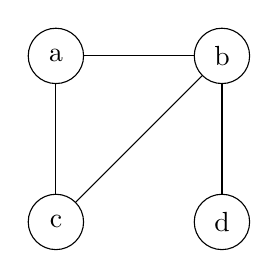
\begin{tikzpicture}
        \tikzstyle{every node}=[draw,circle,minimum size = 2em,node distance = 6em]
        \node (a) {a};
        \node [right of = a] (b) {b} edge(a);
        \node [below of = a] (c) {c} edge(a) edge(b);
        \node [below of = b] {d} edge(b);
    \end{tikzpicture}
\end{figure}

The adjacency matrix and adjacency list for \cref{example_graph} would be:
\begin{table}[ht!]
\begin{minipage}[b]{0.56\linewidth}
\centering
    \begin{tabular}{l|llll}
        & A & B & C & D \\ \hline
         A & 0  & 1  & 1  & 0  \\
         B & 1  & 0  & 1  & 1  \\
         C & 1  & 1  & 0  & 0  \\
         D & 0  & 1  & 0  & 0  \\
    \end{tabular}
    \caption{Adjacency Matrix}
    \label{table:student}
\end{minipage}\hfill
\begin{minipage}[b]{0.4\linewidth}
\centering
\begin{tikzpicture}
    \matrix (M) [matrix of nodes,
                column sep=-\pgflinewidth,
                row sep=0pt,
                nodes in empty cells,
                nodes={draw,fill=gray!20,minimum width=.5cm,outer sep=0pt,minimum height=.7cm,anchor=center},
                column 1/.style={minimum height=.8cm, minimum width=2em}]{
        a &[8mm] b & \mbox{} &[4mm] c & /       \\
        b & a      & \mbox{} & c      & \mbox{}  & [4mm]d    & /  \\
        c & a      & \mbox{} & b      & /         \\
        d & b      & \mbox{} & /      & \mbox{}  \\
    };
    \foreach \i in {1,2,3,4}{
        \path (M-\i-1) [late options={label=left:\i}];
        \draw[->] (M-\i-1.east)--(M-\i-2.west);
        \draw[->] (M-\i-3.center)--(M-\i-4.west);
    }
    \draw[->] (M-2-5.center)--(M-2-6.west);
\end{tikzpicture}
\captionof{figure}{Adjacency List}
\label{fig:image}
\end{minipage}
\end{table}

The running time for these two data structures are shown in
\cref{table:running_time_of_amaj}.

\begin{table}[H]
    \caption{Running Time Analysis for Adjacency Matrix and Adjacency List}
    \label{table:running_time_of_amaj}
    \centering
    \begin{tabular}{l|c|c}
        \hline
        Time & Adjacency Matrix & Adjacency List \\\hline
        visit neighbor & \bigO{1} & \bigO{1}\\
        visit all neighbors & \bigO{n} & \bigO{degree(v)} \\
        test if $uv \in E$ & \bigO{1} & \tikzmark{runanaadaj1}{\bigO{degree(v)}}\\
        add/delete edge & \bigO{1} & \tikzmark{runanaadaj2}{\bigO{n}}\\
        size & \bigO{mn} & \bigO{m+n}
    \end{tabular}
    \begin{tikzpicture}[remember picture,overlay,node distance = 1cm]
        \node[below right = 4em and 1em of runanaadaj1] (notes) {\bigO{1} with hashing.};
        \draw[->,thick] (runanaadaj1.east) to [in=90,out=0] (notes.north);
        \draw[->,thick] (runanaadaj2.east) to [in=90,out=0] (notes.north);
    \end{tikzpicture}
\end{table}


\subsection{Traversing Graph}
\subsubsection{Intuitive Approach}
Assume $G$ is a connected, undirected graph.
Suppose we want to visit every vertex in $G$,
we can use Depth First Search (DFS) is a recursive
manner, as shown in \cref{algo:recursiveDFS}.

\begin{algorithm}[H]
    \caption{Recursive Depth First Search Algorithm}\label{algo:recursiveDFS}
    \begin{algorithmic}[1]
        \Procedure{RecursiveDFS}{$v$}
            \If{$v$ unmarked}
                \State Mark $v$.\Comment{has $v$ been visited.}
                \For{each edge $vw$.}
                    \State\ProcedureName{RecursiveDFS}{w}
                \EndFor
            \EndIf
        \EndProcedure
    \end{algorithmic}
\end{algorithm}

Initially, call \ProcedureName{RecursiveDFS}{s},
where $s \in V$ is some start vertex.

Note that the functions was called recursively, forming an implicit stack.
We can re-write as an iteration using an explicit stack,
as shown in \cref{algo:iterativeDFS}.

\begin{algorithm}[H]
    \caption{Iterative Depth First Search Algorithm}\label{algo:iterativeDFS}
    \begin{algorithmic}[1]
        \Procedure{IterativeDFS}{$s$}
            \State\ProcedureName{Push}{s}
            \While{stack not empty}
                \State $s = \ProcedureName{Pop}{}$
                \If{$v$ is unmarked.}
                    \State Mark $v$.
                    \For{each edge $vw$.}
                        \If{$w$ is unmarked.}
                            \Comment{This \emph{if} is optional in some cases.}
                            \State\ProcedureName{Push}{w}
                        \EndIf
                    \EndFor
                \EndIf
            \EndWhile
        \EndProcedure
    \end{algorithmic}
\end{algorithm}

\observation
Traversal algorithms store candidate vertices in a ``bag'',
which can be any structure allowing insertion/deletion.

\subsubsection{Generic Traverse Algorithm}

So we can define this generic traverse algorithm
as shown in \cref{algo:genericTraverse}.


\begin{algorithm}[H]
    \caption{Generic Traverse Algorithm}\label{algo:genericTraverse}
    \begin{algorithmic}[1]
        \Procedure{Traverse}{$s$}
            \State Put $s$ in bag.
            \While{Bag is not empty.}
            \State \tikzmark{algogenericTraverseambiguousPoint}{Take $v$ from bag.}
                \If{$v$ is unmarked.}
                    \State Mark $v$.
                    \For{each edge $vw$.}
                        \If{$w$ is unmarked.}
                        \Comment{\tikzmark{algogenericTraverseNote}{This \emph{if} is optional in some cases.}}
                            \State Put $w$ in bag.
                        \EndIf
                    \EndFor
                \EndIf
            \EndWhile
        \EndProcedure
    \end{algorithmic}
    \begin{tikzpicture}[remember picture,overlay,node distance = 1cm]
        \node[above right = 0em and 8em of algogenericTraverseambiguousPoint] (notes)
            {\textbf{This step is ambiguous.}};
        \draw[blue,->,thick] (algogenericTraverseambiguousPoint.east) to [in=180,out=0] (notes.west);
        \node[below = 3em of algogenericTraverseNote, text width=8cm] (notes1)
            {In other application, this line may bot be needed, as for traversing, it is needed.};
        \draw[blue,->,thick] (algogenericTraverseNote) to (notes1);
    \end{tikzpicture}
\end{algorithm}

\observation This traverse algorithm clearly marks each vertex at most once.
Now we want to prove it marks each vertex at least once,
i.e. ``visit'' every vertex. To do this, we can remember each vertex's
parent in the process. The modified algorithm is shown in \cref{algo:genericTraverseM}


\begin{algorithm}[H]
    \caption{Remember Parent version of Generic Traverse Algorithm}\label{algo:genericTraverseM}
    \begin{algorithmic}[1]
        \Procedure{Traverse}{$s$}
            \State Put $(\varnothing,s)$ in bag.
            \While{Bag is not empty.}
                \State Take $(p,v)$ from bag.
                    \Comment{\bigO{1} per round.}
                \If{$v$ is unmarked.}
                \Comment{\bigO{m} overall, regardless of inner \emph{for}.}
                    \State Mark $v$.
                    \State $Parent(v) = p$
                    \For{each edge $vw$.}
                            \Comment{\bigO{m} overall.}
                        \If{$w$ is unmarked.}
                            \State Put $(v,w)$ in bag.
                        \EndIf
                    \EndFor
                \EndIf
            \EndWhile
        \EndProcedure
    \end{algorithmic}
\end{algorithm}

\begin{lemma}
    \ProcedureName{Traverse}{s} marks every vertex in connected graph exactly once.

    Set of pair $(parent(v),v)$ with $parent \neq \varnothing$ defines spanning tree.
\end{lemma}

\begin{proof}
    $s$ is marked, so let $v \neq s$.

    Let $(s,\ldots,u,v)$ be shortest path from $s$ to $v$, use induction on path length.
    By induction, $u$ is visited, which implies that when $u$ is marked,
    $(u,v)$ is put in the bag.

    Call a pair $(parent(v),v)$, s.t. $parent(v) \neq \varnothing$ a parent edge.
    Consider the path $(v,parent(v),parent(parent(v)),\ldots)$, this path eventually lead to $s$.
    If every vertex has path to $s$, then parent edge define connected spanning graph.
\end{proof}

\vspace{0.1in}\noindent\textbf{Running Time for Generic Traverse Algorithm}

Each vertex marked exactly once. Each edge $(v,w)$ added to bag at most once
by $v$ and at most once by $w$.

Inner loop executed at most \bigO{m} time.
Outer loop \bigO{m} time. In total, \bigO{m} time.

Note that, this running time analysis ignore bag operation
time (consider \bigO{1} for all bag operations). If bag operation
takes $b$ per operation, \bigO{mb} total time is required.

For connected graph, $n = \bigO{m}$.

\subsubsection{Usage of Using Generic Travers Algorithm}
\begin{enumerate}
    \item Bag is stack $\Longrightarrow$ DFS (results in a long skinny tree).
    \item Bag is queue $\Longrightarrow$ BFS (results in a short fat tree).
    \item If edges have weight, and bag is min priority queue on edge weights.\\
        $\Longrightarrow$ MST, Prim's Algorithm.
    \item Bag is min priority queue on vertex distance.\\
        $\Longrightarrow$ Dijkstra's Algorithm, shortest path tree.
\end{enumerate}

If $G$ is disconnected, we can use a wrap functions to traverse,
as shown in \cref{algo:wrapperGenericTraverse}.

\begin{algorithm}[H]
    \caption{Wrapper for Traverse}\label{algo:wrapperGenericTraverse}
    \begin{algorithmic}[1]
        \Procedure{TraverseAll}{}
            \For{all vertices $v$}
                \If{$v$ is unmarked.}
                    \State\ProcedureName{Traverse}{v}
                \EndIf
            \EndFor
        \EndProcedure
    \end{algorithmic}
\end{algorithm}

\begin{lemma}
    \ProcedureName{TraverseAll}{} marks every vertex in disconnected graph exactly once.

    Set of pair $(parent(v),v)$ with $parent \neq \varnothing$ defines spanning forest.
\end{lemma}

\subsection{Standard Graph Algorithm}
\begin{enumerate}[label=Step {\arabic*}, leftmargin=0.5in]
    \item Maintain set $S$ of visited vertices, and $T \setminus S$ of unvisited.
    \item Maintain tree over $S$.
    \item Repeat:
        \begin{enumerate}
            \item Pick vertex $w$ in $T$, which is adjacent to $S$.
            \item Add to $S$, remove from $T$, update tree on $S$.
        \end{enumerate}
\end{enumerate}

\subsection{Depth First Search}
\subsubsection{Formal Definition}
The Formal definition of DFS is shown in \cref{algo:formalDFS}.
\begin{algorithm}[H]
    \caption{Formal Definition of DFS}\label{algo:formalDFS}
    \begin{algorithmic}[1]
        \Procedure{DFS}{$v$}
            \State Mark $v$.
            \For{each edge $vw$.}
                \If{$w$ is unmarked.}
                    \State\ProcedureName{DFS}{w}
                \EndIf
            \EndFor
        \EndProcedure
    \end{algorithmic}
\end{algorithm}

\observation The procedure create a similar stack of that
in \cref{algo:genericTraverse}, but it's the program's stack.
When \ProcedureName{DFS}{w} makes recursive call, it stores
current program on program stack, i.e. when \ProcedureName{DFS}{v}
calls \ProcedureName{DFS}{w}, \ProcedureName{DFS}{v} is on stack.


Given $v$ in undirected $G$, \ProcedureName{DFS}{v} visits
all vertices in $v$'s component.

\begin{algorithm}[H]
    \caption{DFS All the Component}\label{algo:dfsall}
    \begin{algorithmic}[1]
        \Procedure{DFSAll}{$G$}
            \For{all $v \in V$}
                \If{$v$ is unmarked.}
                    \State\ProcedureName{DFS}{v}
                \EndIf
            \EndFor
        \EndProcedure
    \end{algorithmic}
\end{algorithm}

\subsubsection{Count and Label Components}
DFS Algorithm can be modified to count and label all the components.
\begin{algorithm}[H]
\caption{Count and Label the Components}\label{algo:countlabel}
    \begin{algorithmic}[1]
        \Procedure{CountAndLabel}{$G$}
            \State $count = 0$
            \For{all $v \in V$}
                \If{$v$ is unmarked.}
                    \State $count = count + 1$
                    \State\ProcedureName{LabelComponent}{v,count}
                \EndIf
            \EndFor
            \Return $count$
        \EndProcedure
        \Procedure{LabelComponent}{$v,count$}
            \State Mark $v$.
            \State $component(v) = count$
            \For{each $vw$}
                \If{$w$ is unmarke.}
                    \State\ProcedureName{LabelComponent}{w,count}
                \EndIf
            \EndFor
        \EndProcedure
    \end{algorithmic}
\end{algorithm}

\subsubsection{Pre/Post Order Traverse of Binary Tree}

Originally, the definition are:
\begin{itemize}
    \item Pre-order: visit, recursive call on left, recursive call on right.
    \item Post-order: recursive call on left, recursive call on right, visit.
\end{itemize}

Consider the problem in the view of DFS:
\begin{itemize}
    \item Pre-order: vertices put on stack;
    \item Post-order: vertices taken off from stack.
\end{itemize}

A modified algorithm is shown in \cref{algo:DFSprepost}
\begin{algorithm}[H]
    \caption{Pre/Post Order Based on DFS}\label{algo:DFSprepost}
    \begin{algorithmic}[1]
        \Procedure{DFSAll}{$G$}
            \State $clock = 0$
            \For{all $v \in V$}
                \If{$v$ is unmarked.}
                    \State\ProcedureName{DFS}{v}
                \EndIf
            \EndFor
        \EndProcedure
        \Procedure{DFS}{$v$}
            \State Mark $v$.
            \State \ProcedureName{Previsit}{v}
            \For{each edge $vw$}
                \If{$w$ is unmarked.}
                    \State\ProcedureName{PreVisit}{w}
                \EndIf
            \EndFor
            \State\ProcedureName{PostVisit}{v}
        \EndProcedure
        \Procedure{PreVisit}{$v$}
            \State $pre(v) = clock$
            \State $clock = clock + 1$
        \EndProcedure
        \Procedure{PostVisit}{$v$}
            \State $post(v) = clock$
            \State $clock = clock - 1$
        \EndProcedure
    \end{algorithmic}
\end{algorithm}

\subsubsection{Directed Graphs and Reachability}
\begin{itemize}
    \item For undirected graph, \ProcedureName{DFS}{v} explores the component of $v$.
    \item For directed graph, it is trickier.
        \begin{itemize}
            \item For $v,u$ in directed graph, $u$ is reachable from $v$,
                if directed path from $v$ to $u$.
            \item Let \ProcedureName{Reach}{v} be set of vertices
                reachable from $v$.
            \item If $v \in \ProcedureName{Reach}{v}$, $v$ may or may not be in
                \ProcedureName{Reach}{u}.
        \end{itemize}
\end{itemize}


\subsection{Directed Acyclic Graphs}
\subsubsection{Definition of DAG}
A \textbf{DAG} is a directed graph with no directed cycles.
\begin{itemize}
    \item For a DAG, if $u \in \ProcedureName{Reach}{v}$,
        then $v \notin \ProcedureName{Reach}{u}$.
    \item A source is a vertex with no incoming edges.
    \item A sink is a vertex with no outgoing edges.
    \item Every DAG has at least one source and at least one sink.
    \item Checking if graph is a DAG need \bigO{n+m} time using DFS.
\end{itemize}
To make concept simpler:
\begin{itemize}
    \item Let $G$ be a directed graph.
    \item $G^\prime$ obtained by adding source $s$, a directed edge from
        $s$ to all vertices of $G$.
    \item $G$ is a DAG $\iff$ $G^\prime$ is a DAG (if and only if).
\end{itemize}

\subsubsection{Algorithm to Determine a DAG}
To illustrate is a program manner,consider 3 status during the traversal.
\begin{itemize}
    \item \textsc{New}: never been of program stack;
    \item \textsc{Active}: is currently on the stack;
    \item \textsc{Done}: is off stack, but was previously on.
\end{itemize}
Thus, the DFS algorithm can be modified as shown in \cref{algo:acyclicDFS}

\begin{algorithm}[H]
    \caption{Determine Whether a Graph is DAG}\label{algo:acyclicDFS}
    \begin{algorithmic}[1]
        \Procedure{IsAcyclic}{$G$}
            \State Add vertex $s$.
            \For{all $v \neq s$ in $V$}
                \State Add edge $s \rightarrow v$.
                \State \ProcedureName{Status}{v} = \textsc{New}
            \EndFor
            \Return \ProcedureName{IsAcyclicDFS}{s}
        \EndProcedure
        \Procedure{IsAcyclicDFS}{$s$}
            \State \ProcedureName{Status}{v} = \textsc{Active}
            \For{each edge $v \rightarrow w$}
                \If{\ProcedureName{Status}{w} = \textsc{Active}}
                    \Return False
                \ElsIf{\ProcedureName{Status}{w} = \textsc{New}}
                    \If{\ProcedureName{IsAcyclicDFS}{w} = False}
                        \Return False
                    \EndIf
                \EndIf
            \EndFor
            \State \ProcedureName{Status}{v} = \textsc{Done}
            \Return True
        \EndProcedure
    \end{algorithmic}
\end{algorithm}

\subsubsection{Proof of Correctness}

Prove ``False'' implies cycle.

Suppose ``False'' is returned, then find edge $v \rightarrow w$
s.t. \ProcedureName{Status}{w} = \textsc{Active}.
\begin{itemize}
    \item If $w$ is \textsc{Active}, then it's on the stack and
        $v$ is currently on top of stack.
    \item If vertex $b$ directly on top of $c$ on stack,
        then there must be an edge $c \rightarrow b$.
    \item Thus there must be a direct path $w \rightarrow \ldots \rightarrow v$,
        appending $v \rightarrow w$ gives a cycle.
\end{itemize}

\noindent Prove cycle leads to ``False''.

Let $w$ be first vertex in cycle that we visit,
$v$ is vertex before $w$ in cycle. Then, there exist a path
$w \rightarrow \ldots \rightarrow v \rightarrow w$.

Since $w$ visited first. \ProcedureName{IsAcyclicDFS}{w}
called first in the cycle.

There is a directed path from $w$ to $v$, so \ProcedureName{IsAcyclicDFS}{v}
is called while $w$ on stack.
During \ProcedureName{IsAcyclicDFS}{v}, $v \rightarrow w$ is looked at.
Thus, result in False.


\subsection{Topological Sort}
Given directed $G$, topological ordering is a total order $\prec$
on the vertices s.t. $u \prec v$ for every edge $u \rightarrow v$.

Informally, a topological sort is the order arranges vertices from
left to right, s.t. all edges go from left to right.
An example is shown in \cref{fig:topoexample}
\begin{figure}[H]
    \caption{Example for Topological Sort}\label{fig:topoexample}
    \centering
    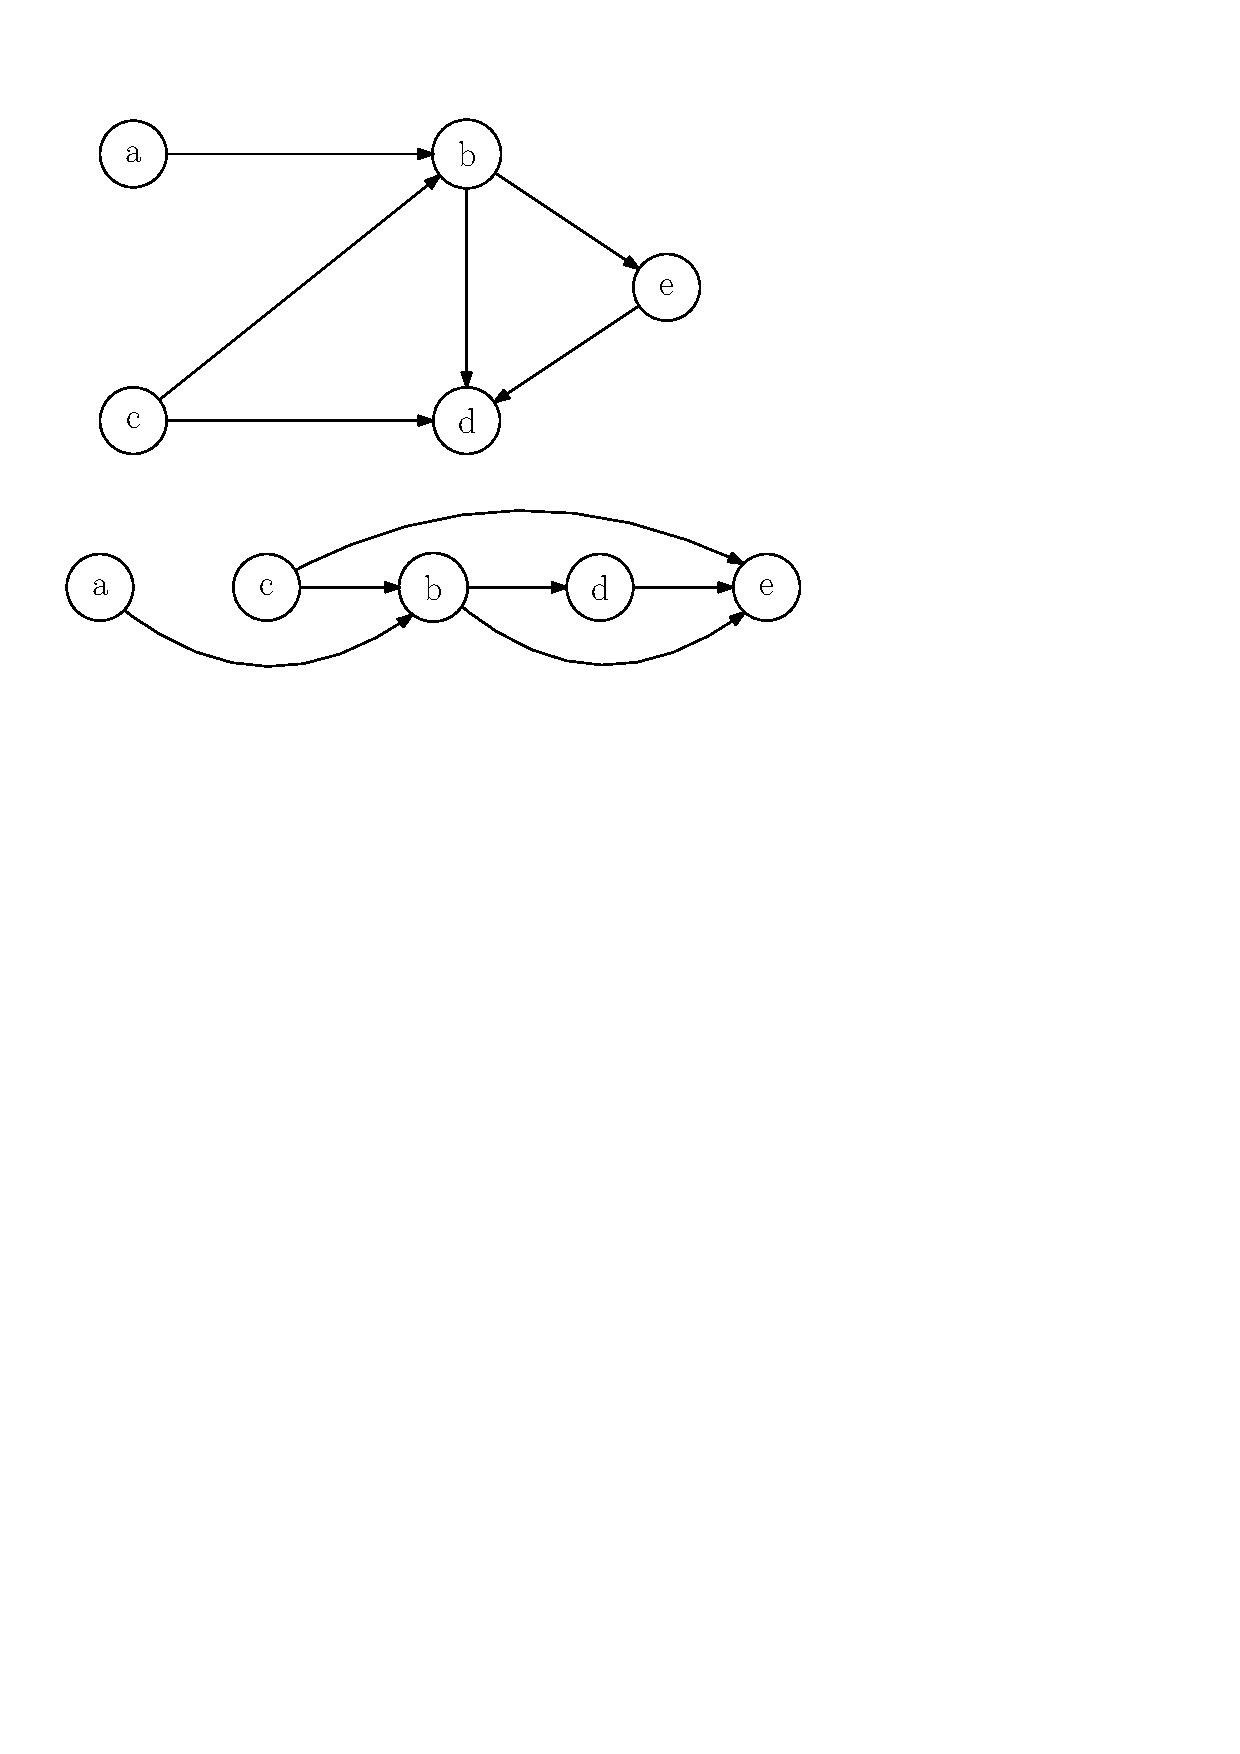
\includegraphics[scale=0.8]{fig/topo1.pdf}
\end{figure}

\observation

The most important fact:
\begin{quote}
$G$ has a topological ordering if and only if no cycles exist,
i.e. $G$ is a DAG.
\end{quote}

A DAG has at least one source/sink, thus the topological sort has
two implementation, one starts from sink, the other starts from source.
The algorithm is shown in \cref{algo:toposink} and \cref{algo:toposource}.

\begin{minipage}[t]{0.48\linewidth}
\vspace{0pt}
\begin{algorithm}[H]
    \caption{Topo-Sort from Source}\label{algo:toposource}
    \begin{algorithmic}[1]
        \Procedure{TopologicalSort}{$G$}
            \State $n = |V|$
            \For{$i = 1 \text{ to } n$}
                \State $v = \text{ any Source }$
                \State $S[i] = v$
                \State Delete $v$
            \EndFor
            \Return $S[1 \ldots n]$
        \EndProcedure
    \end{algorithmic}
\end{algorithm}
\vspace{2pt}
\end{minipage}\hfill
\begin{minipage}[t]{0.48\linewidth}
\vspace{0pt}
\begin{algorithm}[H]
    \caption{Topo-Sort from Sink}\label{algo:toposink}
    \begin{algorithmic}[1]
        \Procedure{TopologicalSort}{$G$}
            \State $n = |V|$
            \For{$i = n \text{ to } 1$}
                \State $v = \text{ any Sink}$
                \State $S[i] = v$
                \State Delete $v$
            \EndFor
            \Return $S[1 \ldots n]$
        \EndProcedure
    \end{algorithmic}
\end{algorithm}
\vspace{2pt}
\end{minipage}

In the algorithm, $v = \text{ any Sink/Source}$ is ambiguous.
Naively, the algorithm takes \bigO{nm} time.

\begin{lemma}
    For any DAG, first vertex marked \textsc{Done} by
    \ProcedureName{IsAcyclic}{} is a sink.
\end{lemma}
\begin{proof}
    Let $v$ be first vertex marked \textsc{Done}. Suppose $v \rightarrow w$ exists.
    \begin{itemize}
        \item If $w$ marked \textsc{Done}, results in contradiction.
        \item If $w$ marked \textsc{Active}, then there is a cycle.
        \item If $w$ marked \textsc{New}, then recursively call on $w$.
            Thus $w$ marked \textsc{Done} before $v$.
    \end{itemize}
    In all three cases, $v$ must be a sink.
\end{proof}

\observation
\begin{itemize}
    \item \ProcedureName{IsAcyclic}{$G$} is modified DFS.
    \item First vertex marked \textsc{Done} is first off stack.
    \item First off stack is the first post order.
    \item This behavior repeats.
\end{itemize}
Thus, Topological order is reverse post order traverse.

Topological ordering computed in \bigO{n+m} time with DFS.

Why does linear time matter?
\begin{itemize}[label={-}]
    \item Scheduling: two jobs $a \rightarrow b$ means
        $a$ depends on $b$.\\
        Reverse topological order is valid job scheduling.
    \item Dynamic Programming.\\
        Recursive sub-problem is a vertex, edges to other sub-problems
        you depend on.
\end{itemize}

\subsection{Strong Connectivity}
$u$ and $v$ are in same strong component if $u \in \ProcedureName{Reach}{v}$
and $v \in \ProcedureName{Reach}{u}$.

Strong Component defines an eequivalent relation.
\begin{itemize}
    \item If $u,v$ in some SC, and $v,w$ in some SC, then
        $u,w$ in same SC.
    \item Define a vertex partition: given two strong components
        $S_1$, $S_2$, $S_1 \cap S_2 = \varnothing$,
        and every vertex in same SC.
\end{itemize}

Denote \ProcedureName{SSC}{G} as Strong Connected Component Graph,
obtained by collapsing each component to vertex, each edge
from $S_1$ to $S_2$, if and only if $\exists u \in S_1, v \in S_2$
s.t. $u \rightarrow v$ in $G$.

\ProcedureName{SSC}{G} is DAG.
In a DAG, every vertex is its own SC.

To compute \ProcedureName{SSC}{G}, call a component sink if sink in
\ProcedureName{SSC}{G}.
Observe that for sink components, \ProcedureName{DFS}{v} for $v \in S$
explores all vertices in $S$.
Thus, the algorithm can be defined as \cref{algo:computeSSC}.

\begin{algorithm}[H]
    \caption{Algorithm to Compute Strong Components}\label{algo:computeSSC}
    \begin{algorithmic}[1]
        \Procedure{StrongComponents}{$G$}
            \State $count = 0$
            \While{$G$ is not empty}
                \State $count = count + 1$
                \State $v = $ any vertex in sink component.
                \State $c = \ProcedureName{DFSLabel}{v,count}$
                \State Remove $c$ from $G$.
            \EndWhile
        \EndProcedure
    \end{algorithmic}
\end{algorithm}

\subsection{Minimum Spanning Tree ( MST )}

\subsubsection{MST Definition}
\AlgoInput Undirected, weighted, connected graph $G$.
Assume there is a function $w:E \rightarrow R$

\AlgoOutput Find the minimum spanning tree of $G$,
i.e. the spanning tree $T$ which minmimizes
$\displaystyle w(T) = \sum_{e \in T} w(e)$.

\subsubsection{MST Property}
Why use MST?

If vertices represent nodes in a network,
and weights represent connection cost.
MST is cheapest way to connect all nodes.

A example of MST is shown in \cref{fig:MSTexample}.
\begin{figure}[ht]
    \caption{Example for MST}\label{fig:MSTexample}
    \centering
    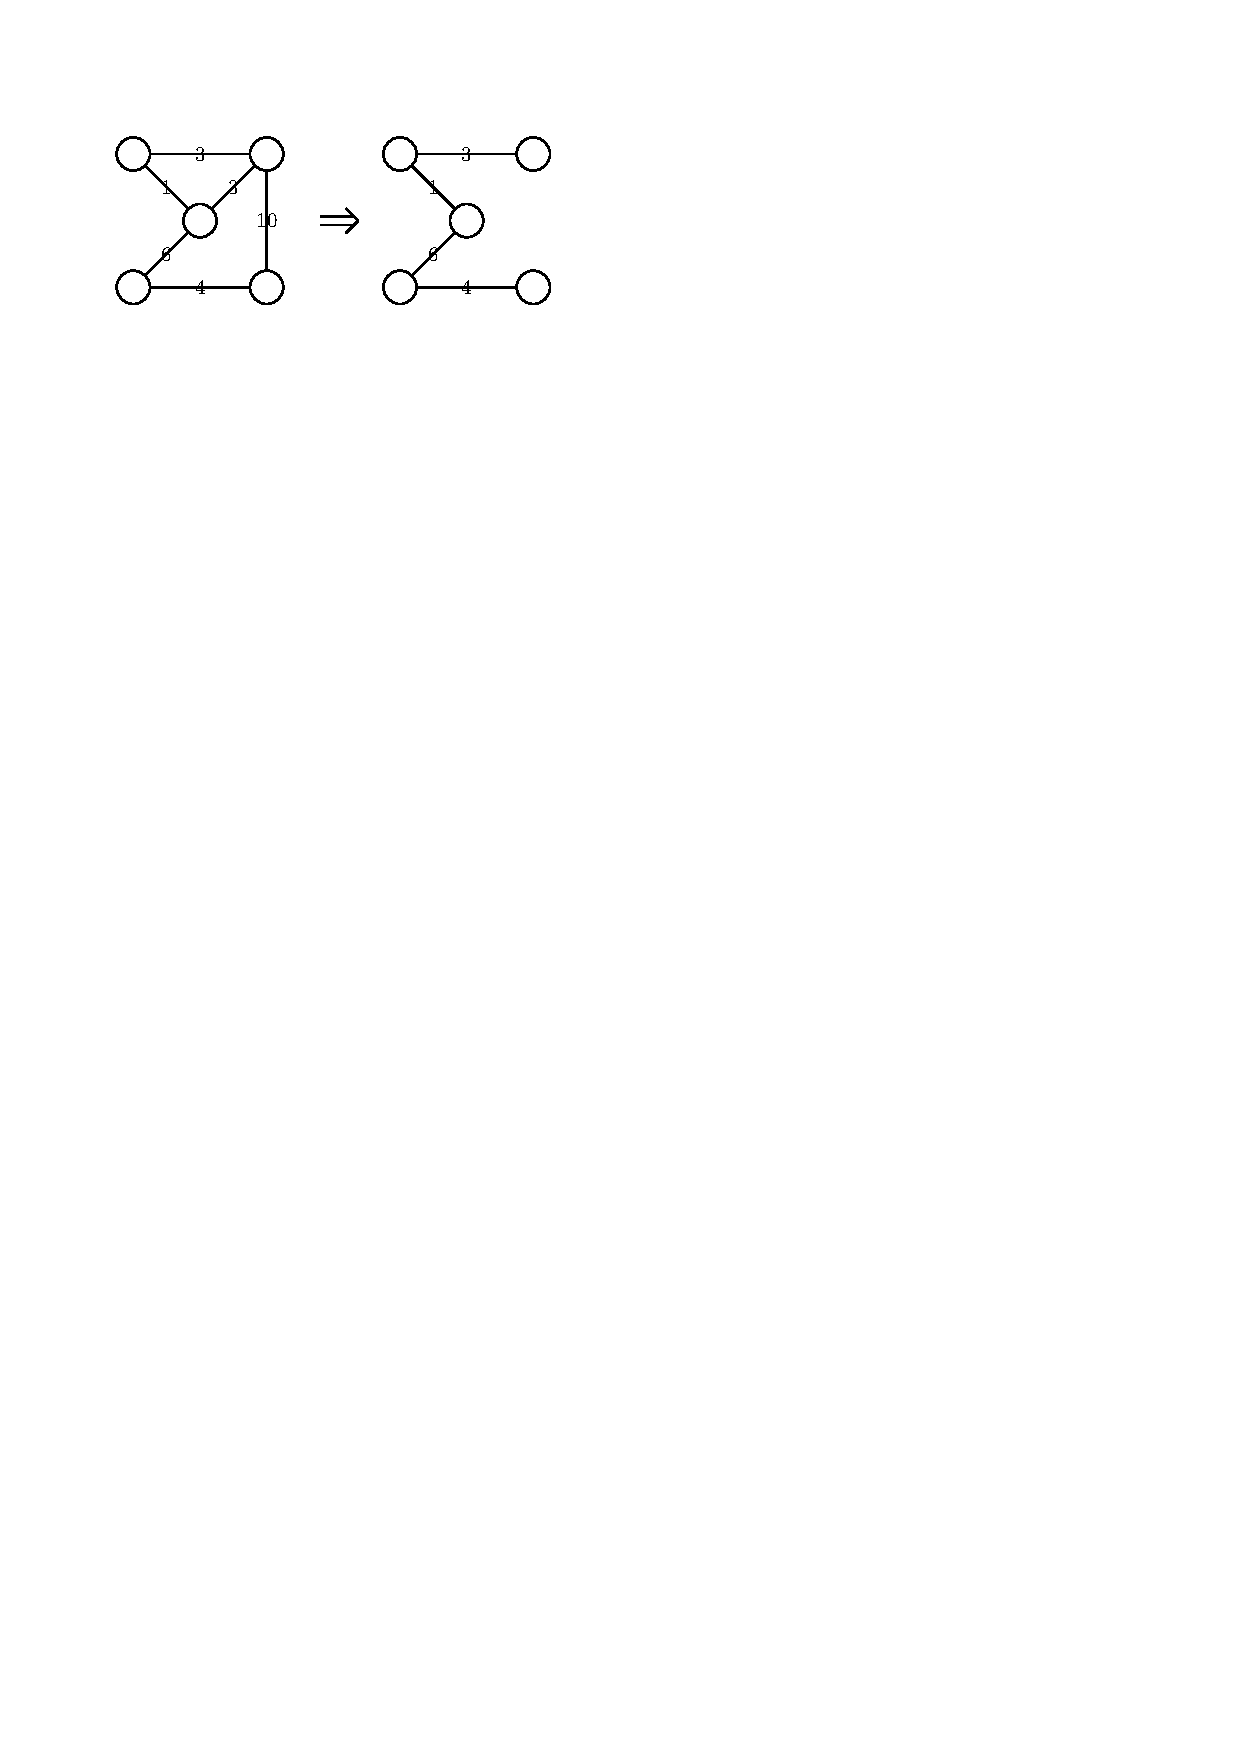
\includegraphics[scale=1.2]{fig/MSTexample}
\end{figure}

\observation

Some properties are obvious:
\begin{itemize}
    \item If all weights distinct, can prove MST is unique.
    \item If all weights equal, any spanning tree is a MST.
\end{itemize}

\noindent \textbf{Main MST Property}

A partition of $V$ is a pair $S,R \subseteq V$,
s.t. $S \cap R = \varnothing$ and $S \cup R = V$.
Given a partition $S,R \subseteq V$, \ProcedureName{mwe}{S,R}
denotes minimum weight edge $u\rightarrow v$, s.t. $u \in S$, $v \in R$.
\begin{itemize}
    \item For any partition $S,R$, $\ProcedureName{mwe}{S,R} \in MST$.
    \item If $e$ is not minimum weight edge of any partition,
        then $e \notin \ProcedureName{MST}{G}$.
\end{itemize}

\begin{proof}
    First, prove that for any partition $S,R$, $\ProcedureName{mwe}{S,R} \in MST$.

    Let $S,R$ be a partition and let $e = \ProcedureName{mwe}{S,R}$.

    Suppose $e = u \rightarrow v$, where $u \in S$, $v \in R$.
    Consider any spanning tree $T$, which does not contain $e$.
    $T$ contains unique path from $u$ to $v$.
    Some edges in this path has endpoint in $S$ and another in $R$.
    Let $e^\prime$ be such an edge.

    Remove $e^\prime$ from $T$, gives a spanning forest, with two trees.
    $u$ and $v$ must be in different trees.

    Hence adding $e$ connects two trees, producing single spanning tree
    $T^\prime = T - e^\prime + e$. $weight(e) < weight(e^\prime)$, so $weight(T^\prime) < weight(T)$.
    $T$ is not MST, result in contradiction.

    Then, prove that if $e$ is not minimum weight edge of some partition,
    then it's not in MST.

    Let $T$ be the MST.
    Consider any edge $e^\prime \in T$. $e^\prime$ define partition of $V$.

    Just proved minimum weight edge across this partition must be in MST.
    Since $e^\prime$ is the only edge in $T$ crossing this partition,
    it must be min weight.
\end{proof}

\subsubsection{MST Algorithm ( General )}
General idea of MST algorithm is:
\begin{quote}
Maintain a spanning forest, initially is $n$ isolated vertices.
Add an edge of MST, update forest, and repeat.
\end{quote}
All the algorithm follows is the variation of this general idea.

\subsubsection{Prim's Algorithm}
\vspace{0.1in}\noindent\textbf{Key point}
\begin{itemize}
    \item Pick vertex $s$. Grow MST from $s$, call it $T$.
    \item In each round, find the edge
        $e = \ProcedureName{mwe}{T, V \setminus T}$.
        Add $e$ to $T$ and repeat.
    \item To find $e$, store edges adjacent to $T$
        in min priority queue.
\end{itemize}
The algorithm is shown in \cref{algo:prim}
\begin{algorithm}[H]
    \caption{Prim's Algorithm}\label{algo:prim}
    \begin{algorithmic}[1]
        \Procedure{Prim}{$s$}
            \State Initial an empty minimum priority queue $Q$.
            \State Mark $s$.
            \For{all edges $s \rightarrow w$}
                \State Put $(s,w)$ in $Q$.
            \EndFor
            \While{$Q$ is not empty}
                \State $(p,v) = Q.pop$
                \If{$v$ is unmarked}
                    \State Mark $v$.
                    \State $\ProcedureName{Parent}{v} = p$
                    \For{each edge $v \rightarrow w$}
                        \State Put $(v,w)$ in $Q$.
                    \EndFor
                \EndIf
            \EndWhile
        \EndProcedure
    \end{algorithmic}
\end{algorithm}

\observation
This traverse with bag = min queue. Marked mean in tree, not in queue.

An example is shown in \cref{fig:prim}.
\begin{figure}[ht!]
    \caption{Example for MST}\label{fig:prim}
    \centering
    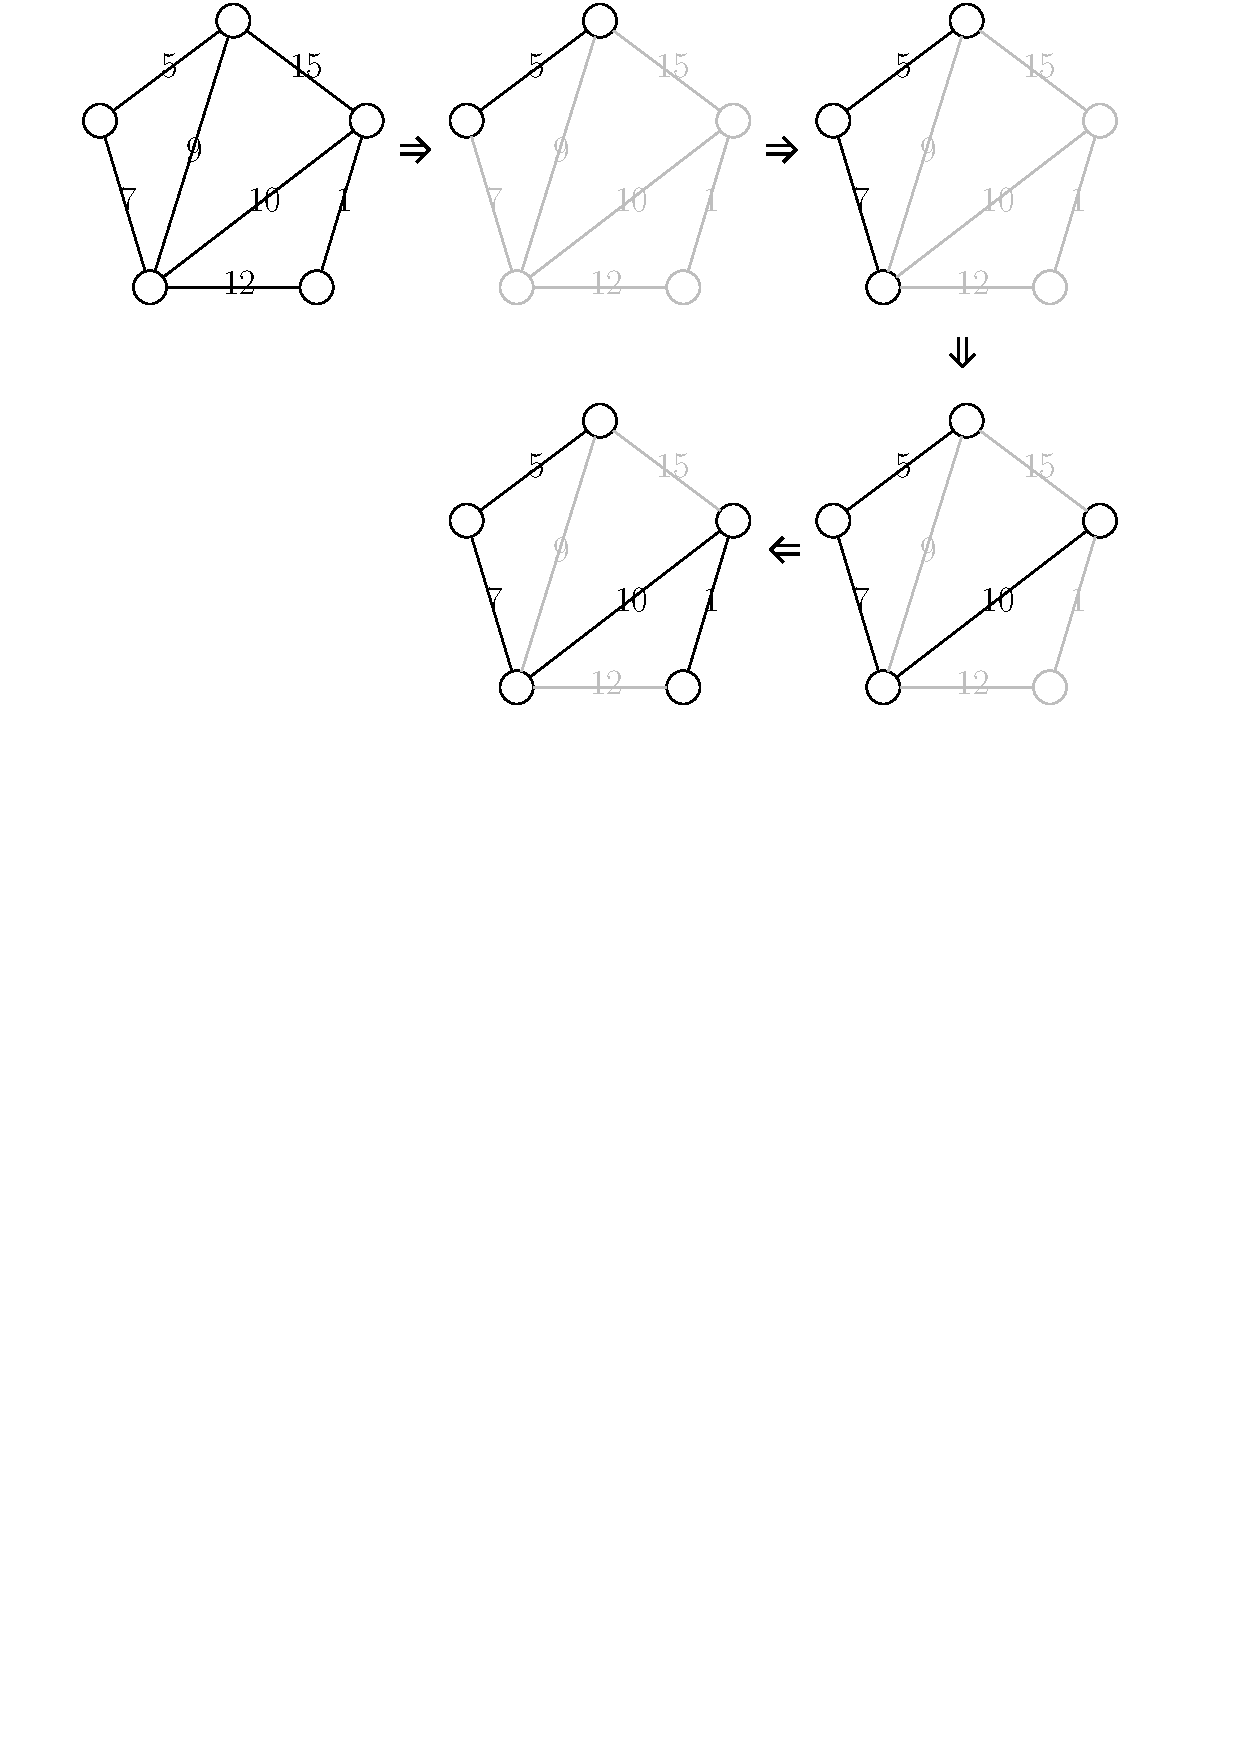
\includegraphics[width=.6\linewidth]{fig/PrimExample}
\end{figure}

\analysis

Each time add \ProcedureName{mwe}{T, V \setminus T},
which we know is in MST, so correct.

Recall that for traverse, running time depend on bag operation cost.
Specifically each edge is added/renewed from $Q$ once,
and this dominates runtime.

If $Q$ implemented in binary min heap, all operations take
\[\bigO{\lg{heap size}} = \bigO{\log(m)} = \bigO{\log(n)}\]
time. Thus total time is \bigO{m \log n}

Note that the running time can be improved to
\bigO{m + n\log n} time using Fibonacci Heap, see Jeff's note.

\subsubsection{Borvka's Algorithm}
\vspace{0.1in}\noindent\textbf{Key point}
\begin{itemize}
    \item Start with forest of singletons, $F = (v,\varnothing)$.
    \item Repeat until $F$ is a single tree:
        For every $T \in F$, add \ProcedureName{mwe}{T, V \setminus T}.
\end{itemize}
The algorithm is shown in \cref{algo:borvka}
\begin{algorithm}[H]
    \caption{Borvka's Algorithm}\label{algo:borvka}
    \begin{algorithmic}[1]
        \Procedure{Borvka}{$V,E$}
            \State $F = (V, \varnothing)$
            \State $count = \ProcedureName{CountAndLabel}{F}$
            \While{$count > 1$}
                \State \ProcedureName{AddAllMWE}{E,F,count}
                \State $count = \ProcedureName{CountAndLabel}{F}$
            \EndWhile
            \Return $F$
        \EndProcedure
        \State
        \Procedure{AddAllMWE}{$E,F,count$}
            \For{$i = 1 \text{ to } count$}
            \State $S[i] = NULL$ \Comment{ $w(null) = \infty$ }
            \EndFor
            \For{each edge $uv \in E$}
                \If{$label(u) \neq label(v)$}
                    \If{$weight(uv) < w(S[label(u)])$}
                        \State $S[label(u)] = uv$
                    \EndIf
                    \If{$weight(uv) < w(S[label(v)])$}
                        \State $S[label(v)] = uv$
                    \EndIf
                \EndIf
            \EndFor
            \For{$i = 1 \text{ to } count$}
                \If{$S[i] \neq NULL$}
                    \State add $S[i]$ to $F$
                \EndIf
            \EndFor
        \EndProcedure
    \end{algorithmic}
\end{algorithm}

$S[i]$ stores minimum weight edge with exactly one endpoint in tree $i$.

\analysis

The algorithm is correct since add \ProcedureName{mwe}{T, V \setminus T}
for each $T \in F$.

The running time:
\begin{itemize}
    \item \ProcedureName{CountAndLabel}{F} takes \bigO{n} time,
        since $F$ has \bigO{n} edge.
    \item \ProcedureName{AddAllMWE}{} takes \bigO{m} time,
        since $\bigO{m + n} = \bigO{m}$.
    \item While-loop takes \bigO{m+n} = \bigO{m} per iteration,
        in total performs \bigO{\lg n} iterations.
\end{itemize}
Thus, total running is \bigO{m\log n}.

\subsubsection{Kruskal's Algorithm}

\vspace{0.1in}\noindent\textbf{Key point}
\begin{itemize}
    \item Sort edges in increasing weight order.
    \item Go through edges in increasing order,
        add edge $e$ if its endpoints in different trees.
\end{itemize}

\vspace{0.1in}\noindent\textbf{Correctness}
1
Suppose we add $e$ joing $T_1,T_2 \in F$,
then $e$ must be \ProcedureName{mwe}{T_1, V \setminus T_1}.
If not, then there was cheaper edge $e^\prime$,
but in which case, $e^\prime$ should be add first.

The difficulty is maintaining $F$.
For Borvka, spend \bigO{m} time to update $F$.
Hence, now consider edges one at a time leads to
\bigO{m \times m} = \bigO{m^2} time.

\vspace{0.1in}\noindent\textbf{Union Find}

Union Find is a data structure which can do the following:
\begin{itemize}
    \item \ProcedureName{MakeSet}{V}: make set (i.e. tree in forest)
        with just $V$.
    \item \ProcedureName{Find}{u}: return set id (some vertex in tree).
    \item \ProcedureName{Union}{u,v}: merges sets containing $u$ and $v$.
\end{itemize}
All operation of Union Find take \bigO{\varpropto(n)} time.

The algorithm is shown in \cref{algo:kruskal}

\begin{algorithm}[H]
    \caption{Kruskal's Algorithm}\label{algo:kruskal}
    \begin{algorithmic}[1]
        \Procedure{Kruskal}{$s$}
            \State sort $E$ by increasing weight order
            \State $F = (V, \emptyset)$
            \For{each vertex $v \in V$}
                \ProcedureName{MakeSet}{v}
            \EndFor
            \For{$i = 1 \text{ to }|E|$}
            \State $uv = i\text{th \textbf{heaviest} edge in } E$
                \If{$\ProcedureName{Find}{u} \neq \ProcedureName{Find}{v}$}
                    \State \ProcedureName{Union}{u, v}
                    \State add $uv$ to $F$
                \EndIf
            \EndFor
            \Return $F$
        \EndProcedure
    \end{algorithmic}
\end{algorithm}

\analysis

The running time:
\begin{itemize}
    \item \bigO{m} find operations.
    \item \bigO{n} union operations.
    \item \bigO{n} makeset operations.
\end{itemize}
So other than sorting, total time is \bigO{m\varpropto(n)}.

Sorting takes \bigO{m\log m} = \bigO{m \log n} time,
dominating the total running.

Thus, total running time would be \bigO{m \log n}.

\subsection{Shortest Paths}
\AlgoInput Weighted directed graph $G$ with labeled
source $s$ and target $t$.

\AlgoOutput Find shortest $s-t$ path, i.e. directed
path $P$ from $s$ to $t$ that minimized
\[w(P) = \sum_{w \rightarrow v \in P}w(u \rightarrow v)\]

Note that we can allow negative weights,
but cannot be negative cycles.

A example is shown in \cref{fig:spexample}.

\begin{figure}[ht!]
    \caption{Example for Shortest Path}\label{fig:spexample}
    \centering
    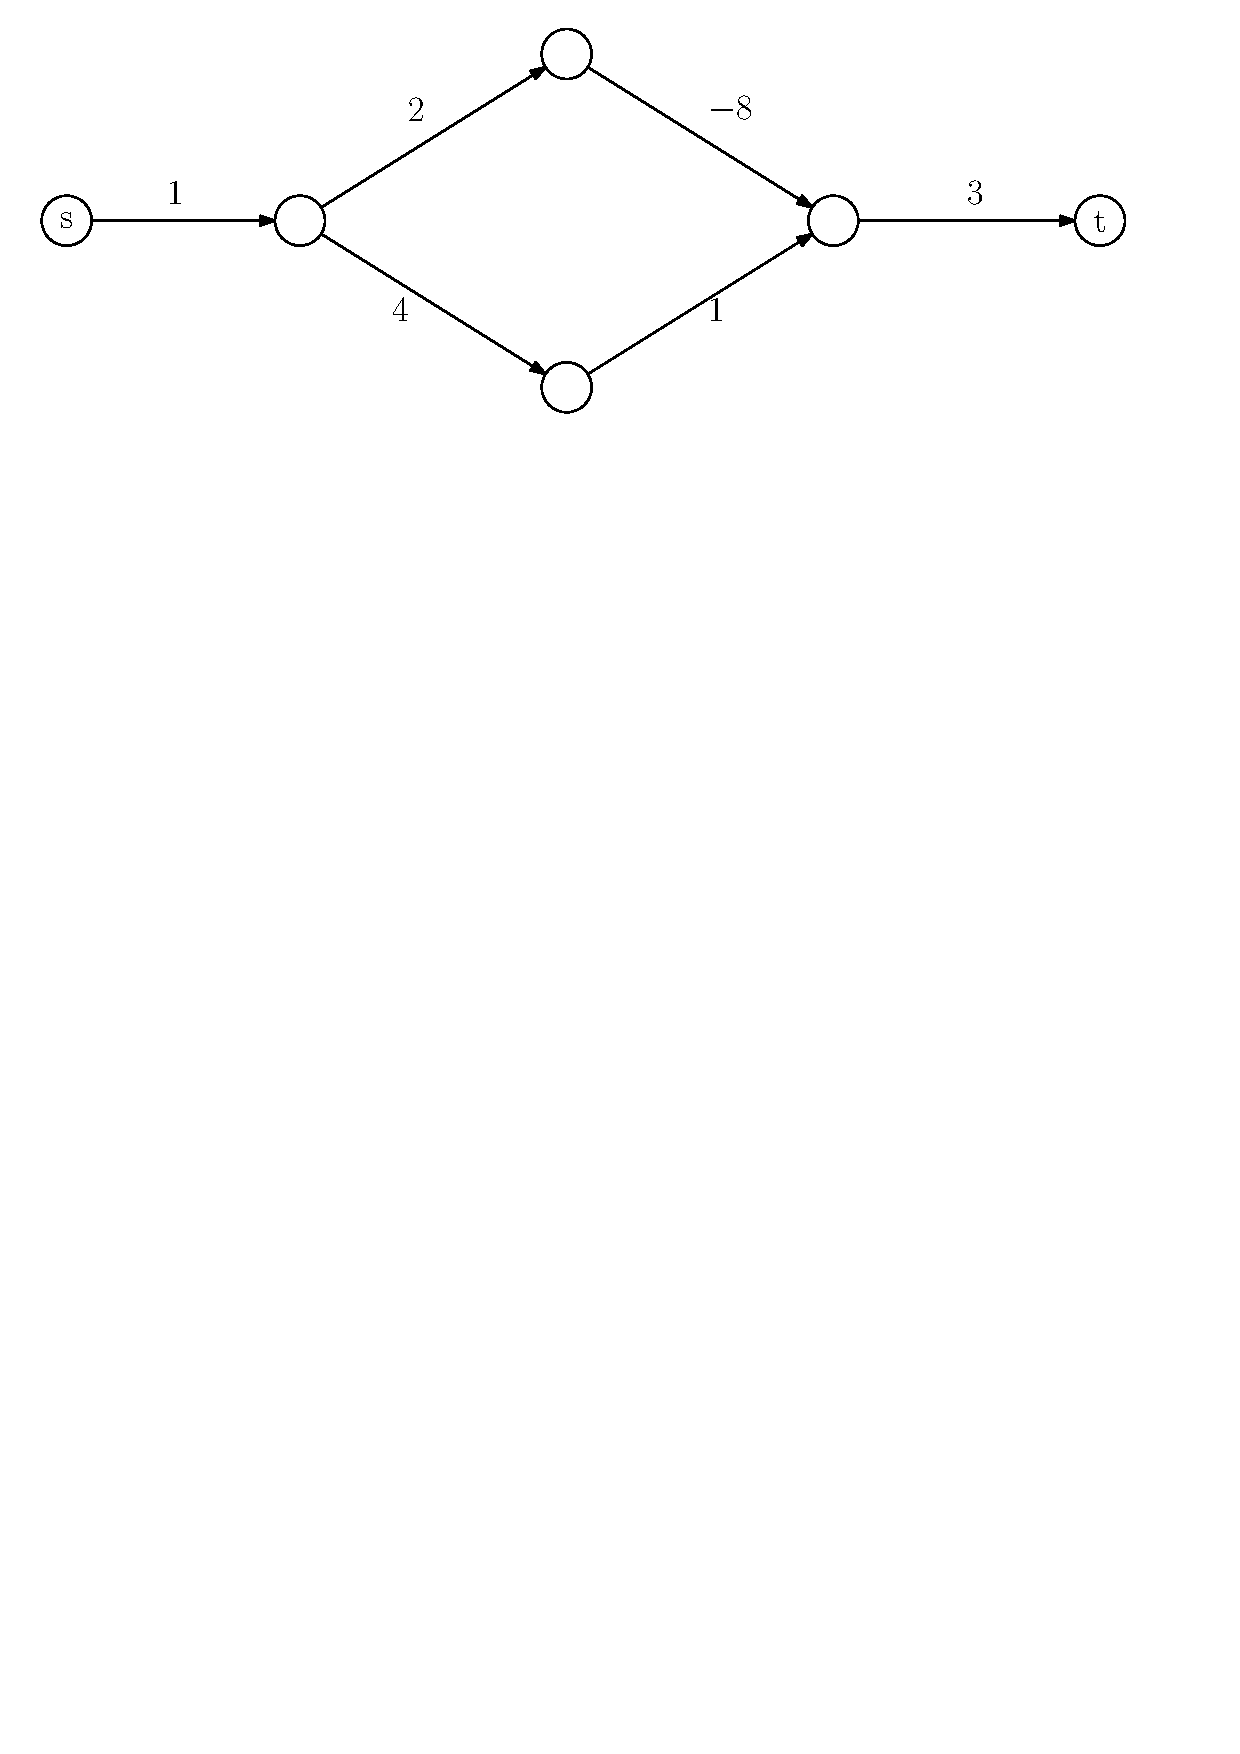
\includegraphics[width=.9\linewidth]{fig/spExample}
\end{figure}

\subsubsection{Single Source Shortest Path ( SSSP )}
Almost every algorithm to find shortest $s-t$ path find
shortest path to every vertex. 

We can represent all shortest paths from $s$ using
a spanning tree rooted at $s$.

Why a tree satisfied?

Suppose shortest $s-w$ path passes through $v$
and shortest $s-t$ path passes through $v$.
The subpath of a shortest path is a shortest path.


\pagebreak

\section{NP-Hardness}

\subsection{A Game You Can't Win}
Given a box with $n$ binary switches and a light bulb.
Inside the box is a boolean circuit, s.t
\begin{itemize}
    \item \textsc{And}, \textsc{Or}, \textsc{Not} gates, as shown in \cref{fig:gates};
    \item $n$ input wires, one per switch;
    \item Gates connected to single output, i.e the light bulb.
\end{itemize}
\begin{figure}[H]
    \centering
    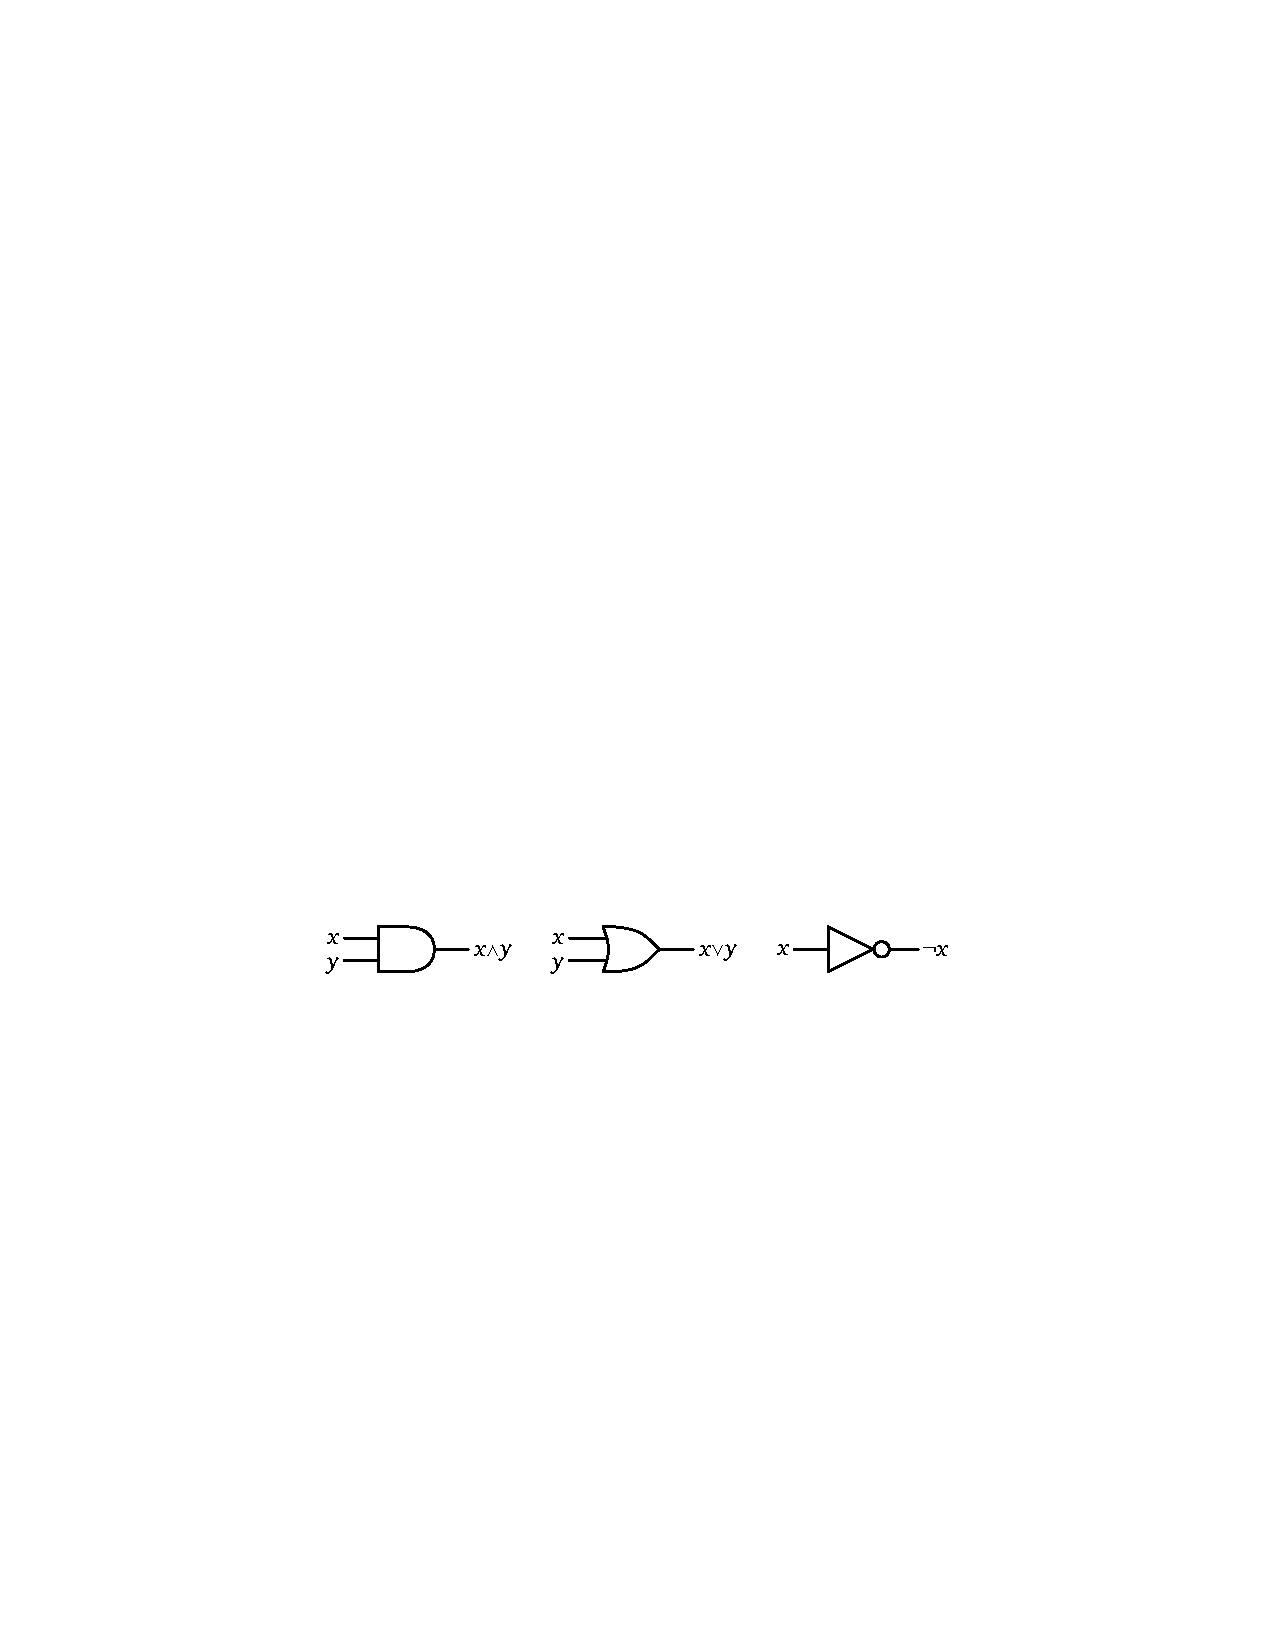
\includegraphics{fig/gates}
    \caption{An \textsc{And}, an \textsc{Or}, and a \textsc{Not} gate}
    \label{fig:gates}
\end{figure}
An example is shown in \cref{fig:lightbulb}
\begin{figure}[H]
    \centering
    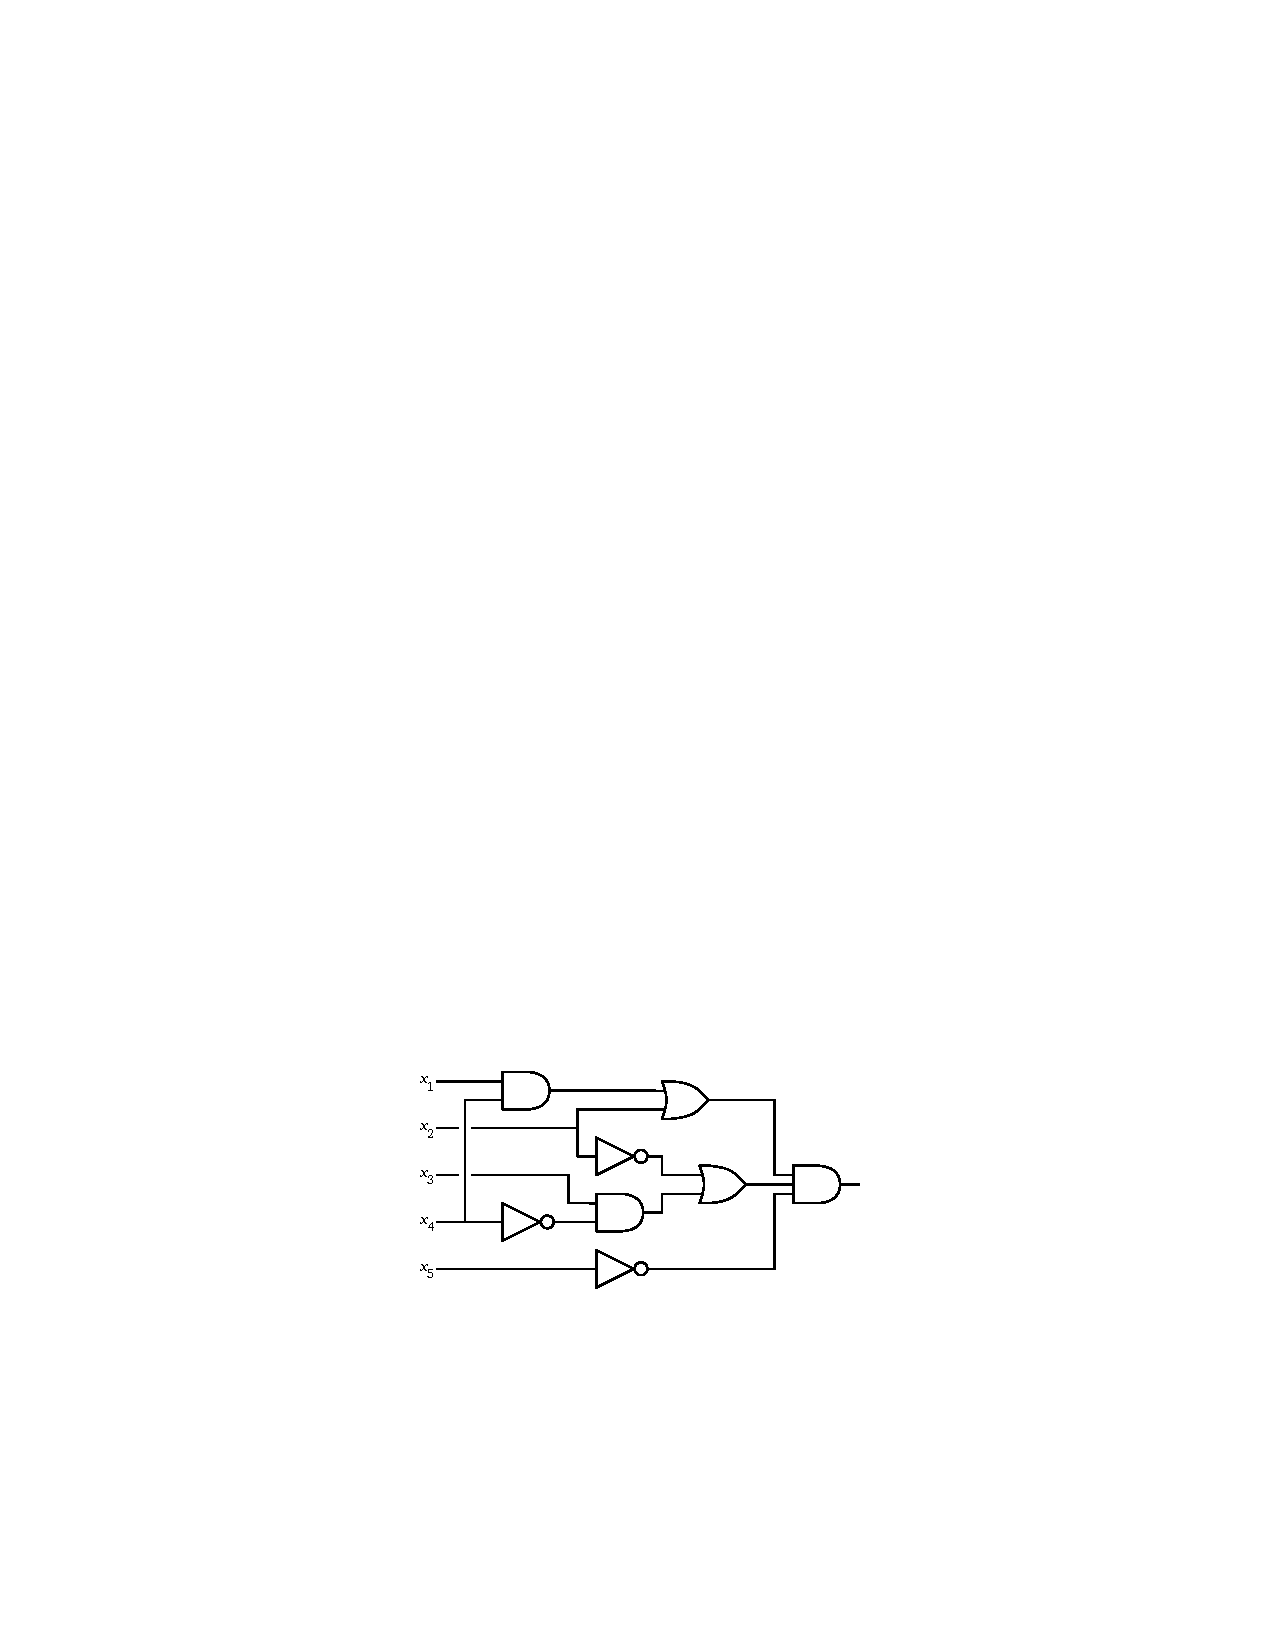
\includegraphics[scale=1.5]{fig/lightbulb}
    \caption{A boolean circuit}
    \label{fig:lightbulb}
\end{figure}
We want to know if there is a way to set switches s.t
light bulb turns on.
There are $2^n$ possible binary inputs. There is an \bigO{n} size circuit
which accepts a single strings and rejects all others.
Hence, if you cannot see inside, in worst case you must try all $2^n$ strings.

Suppose now you can see inside box. Can you do better than guessing all strings?
The answer is nobody knows for sure but many believe not.

The problem of determining if boolean circuit has satisfying assignment is all
\textsc{CircuitSAT}.

\subsection{P versus NP}
Minimum for an algorithm to be efficient is that it runs in polynomial time,
i.e \bigO{n^c} for constant $c$, $n$ is input size.
In this course, we focused on problems with polynomial solutions where $c$ is small.
\begin{itemize}
    \item Some problems known to require exponential time, i.e \bigO{c^n}, $c>1$.
    \item Some problems cannot even be solved (for example, Halting Problem).
    \item Some problems we don't know how hard.
\end{itemize}
NP-hard is a class most believe cannot be solved in polynomial time,
but no one knows for sure.

A decision problem is a problem whose output is a single boolean value,
i.e. \textsc{Yes/No}.
For example: LIS was an optimization problem. $\rightarrow$ ``Is there any increasing sequence of length $\geq k$?''
is a decision problem.
\begin{itemize}[leftmargin=.75in]
    \item[P] Set of decision solvable in polynomial time, i.e ``efficiently solvable''.
    \item[NP] Decision problems s.t if answer in \textsc{Yes}, then there is a proof
        that can be checked in polynomial time. $\rightarrow$ can verify \textsc{Yes} if proof given to us.
    \item[Co-NP] Decision problems s.t if answer in \textsc{No}, then there is a proof
        that can be checked in polynomial time. $\rightarrow$ can verify \textsc{No} if proof given to us.
\end{itemize}
\textsc{CircuitSAT} is in NP, if satisfying string, then given string, it is easy to verify.

Why do most believe $P \neq NP$?
One intuition is that: solving problems is harder than verifying solutions.
\begin{itemize}[leftmargin=.75in]
    \item[P] Problem in CLRS that you can solve quickly.
    \item[NP] Problem in CLRS that you can verify solution quickly.
\end{itemize}

\subsection{NP-Hard/NP-Complete}
A problem $\Pi$ is NP-hard if a polynomial time algorithm for $\Pi$ implies
polynomial time algorithm for all problems in NP.
\begin{quote}
    $\Pi$ is NP-hard $\leftrightarrow$ If $\Pi$ solution in polynomial time, then P = NP.
\end{quote}

Hence, most believe no NP-hard problem solvable in polynomial time.

$\Pi$ is NP-complete if $\Pi$ is NP-hard and $\Pi \in \text{NP}$.

Thousands of problems have been shown to be NPC.
How does one prove something NP-hard or NPC?

\begin{theorem}[Cook-Levin Theorem] \textsc{CircuitSAT} is NPC.\end{theorem}

All problems that are shown to be NPC, reduce from \textsc{CircuitSAT}.

\subsection{Reductions \& SAT}
To prove any problem other than the \textsc{CircuitSAT} is NP-hard, use reduction.
Reducing problem A to problem B means solving A using solution for B.
To prove B is NP-hard, reduce \underline{from} known NP-hard problem A \underline{to} problem B.
Require reduction to be polynomial time in the A instance size.

Intuition: we are sure A is hard, Hence B must be hard, since otherwise it implies A can be
solved quickly.

Often write: $B \geq_p A$,
$\geq_p$ stands for B at least as hard as A ignoring polynomial factor.

A may still require more time to solve bu not more than polynomial factor.

Given a boolean formula, is there a satisfying assignment,
i.e a binary assignment variables evaluating to be true.
For example: 
\[(a \lor b \lor c \lor \overline{d}) \Longleftrightarrow ((b \land \overline{c}) \lor \overline{(\overline{a} \Rightarrow d)} \lor (c \neq a \land b))\]
To prove SAT is NP-hard, we reduce from \textsc{CircuitSAT}.
So given a boolean circuit (i.e. a DAG), we must convert to an equivalent boolean formula.

One solution: circuit has single output gate,
so start at root gate, recursively write formula,
for each subtree and combine formula with root gate operation.
This method takes exponential time since DAG, not a tree.

Here is the polynomial time reduction:
\begin{enumerate}
    \item For each gate output wire create a variable: $y_1 \ldots y_n$ as gates outputs,
        $x_1 \ldots x_m$ as circuit input, $z$ as circuit output.
    \item For each gate wire clause saying inputs match output.
    \item Take \textsc{And} of all these clauses and $z$.
    \item This says all gates work properly and output is $1$.
\end{enumerate}
For example, \cref{fig:sat} shows the formula transformed from \cref{fig:lightbulb}.
\begin{figure}[H]
    \centering
    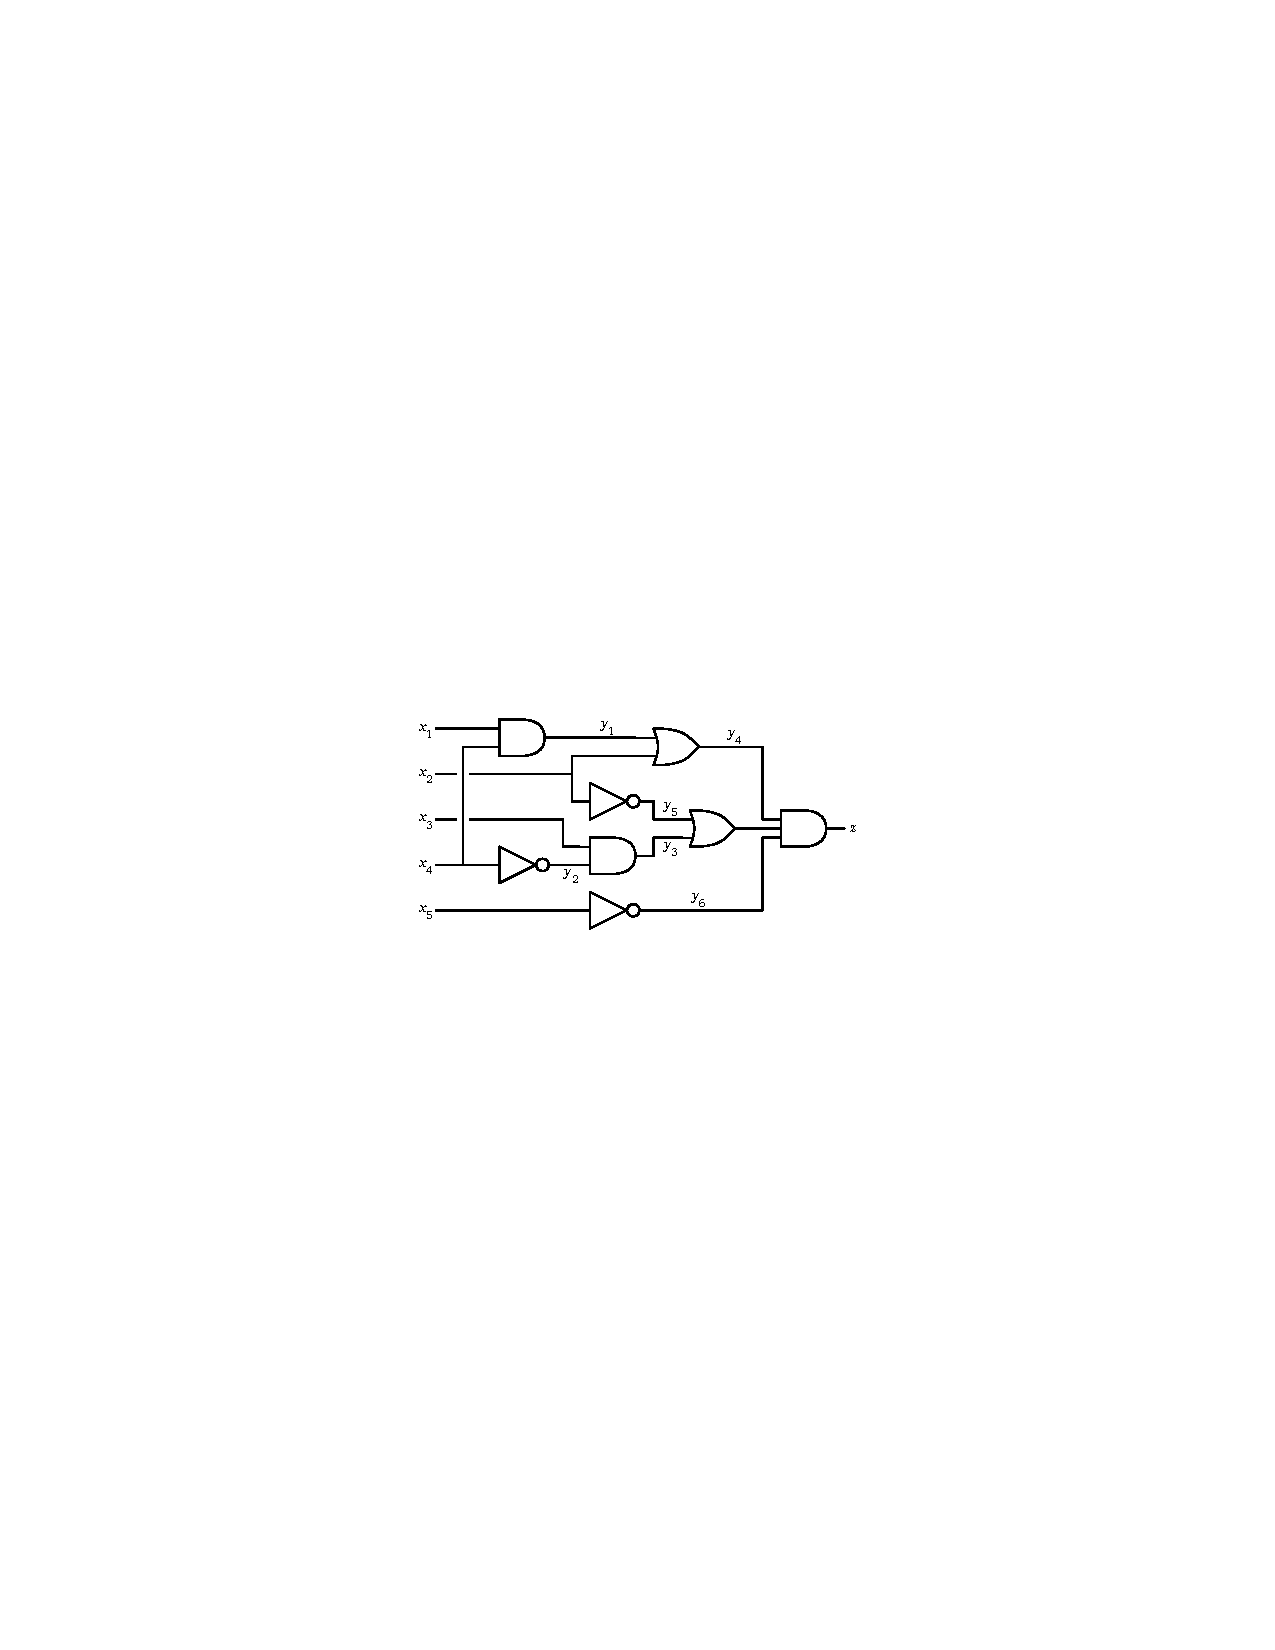
\includegraphics[scale=1.25]{fig/sat}
\begin{align*}
    (y_1 = x_1 \land x_4)\land&(y_2 = \overline{x_4})\land(y_3 = x_3 \land y_2)\land(y_4 = y_1 \land x_2)\land\\
    &(y_5 = \overline{x_2})\land(y_6 = \overline{x_5})\land(y_7 = y3 \lor y_5)\land(z = y_4 \land y_7 \land y_6) \land z
\end{align*}
    \caption{A boolean circuit with gate variables added, and an equivalent boolean formula}
    \label{fig:sat}
\end{figure}
The original circuit is satisfiable if and only if the boolean formula is.
\begin{itemize}[leftmargin=.75in]
    \item[$\Longrightarrow$] Given satisfying assignment to circuit, can find satisfying assignment to formula
        by computing output of every gate.
    \item[$\Longleftarrow$] Given satisfying assignment to formula, just ignore $y_i$s and $z$ to get circuit input.
\end{itemize}
By this, we can produce formula from circuit in linear time.
Thus, polynomial time reduction from \textsc{CircuitSAT} to SAT.

\subsection{3SAT}
Boolean formula is in conjunctive normal form (CNF) if it is the
conjunction (\textsc{And}) of clause,
each of which is a disjunction (\textsc{Or}) of literals,
each of which is a variable of its negation.

A 3CNF formula is a CNF formula with exactly 3 literals per clause.

\begin{theorem}
    3SAT is NP-complete.
\end{theorem}
\begin{proof}
To prove 3SAT $\in$ NP, given satisfying assignment, plug in values and evaluate.

To prove 3SAT is NP-hard: (reduce from \textsc{CircuitSAT})

Given \textsc{CircuitSAT} instance, convert to 3SAT instance:
Assume each gate has fan in at most 2.
\begin{enumerate}
    \item Write circuit as formula with one clause per gate;
    \item Change each gate clause to CNF:
        \begin{align*}
            a=b \land c &\Longleftrightarrow (a \lor \overline{b} \lor \overline{c}) \land
                (\overline{a} \lor b) \land (\overline{a} \lor c) \\
            a=b \lor c &\Longleftrightarrow (\overline{a} \lor b \lor c) \land
                (a \lor \overline{b}) \land (a \lor \overline{c}) \\
            a = \overline{b} &\Longleftrightarrow (a \lor b) \land (\overline{a} \lor \overline{b})
        \end{align*}
    \item Convert to 3CNF (exactly 3 literals per clause)
        \begin{align*}
            a &\Longleftrightarrow (a \lor x \lor y) \land (a \lor \overline{x} \lor y) \land
                (a \lor x \lor \overline{y}) \land (a \lor \overline{x} \lor \overline{y}) \\
            a \lor b &\Longleftrightarrow (a \lor b \lor x) \land (a \lor b \lor \overline{x})
        \end{align*}
\end{enumerate}
Polynomial time reduction, hence 3SAT is NP-hard.
\end{proof}

\subsection{Independent Set}
Let $G$ be an undirected graph. An independent set in $G$ is a set of vertices
with no edge between them.

\noindent\textbf{Independent Set Problem}: Given $G$ and integer $k$, is there an independent set of size $\geq k$.

\noindent\textbf{Max Independent Set Problem}: Given $G$, find the size of largest independent set.

\begin{proof}
We prove the Independent Set Problem is NP-hard by reducing from 3SAT:
Input is a 3SAT instance with $x$ clauses.
For each literal of each clause, create a vertex.
Add an edge between two vertices if either:
\begin{itemize}
    \item literals are in the same clause;
    \item literal correspond to variable and its negation.
\end{itemize}
For example the following formula
\[(a \lor b \lor c) \land (b \lor \overline{c} \lor \overline{d}) \land
    (\overline{a} \lor c \lor d) \land (a \lor \overline{b} \lor \overline{d})\]
is transformed into the following graph:

\begin{figure}[H]
    \centering
    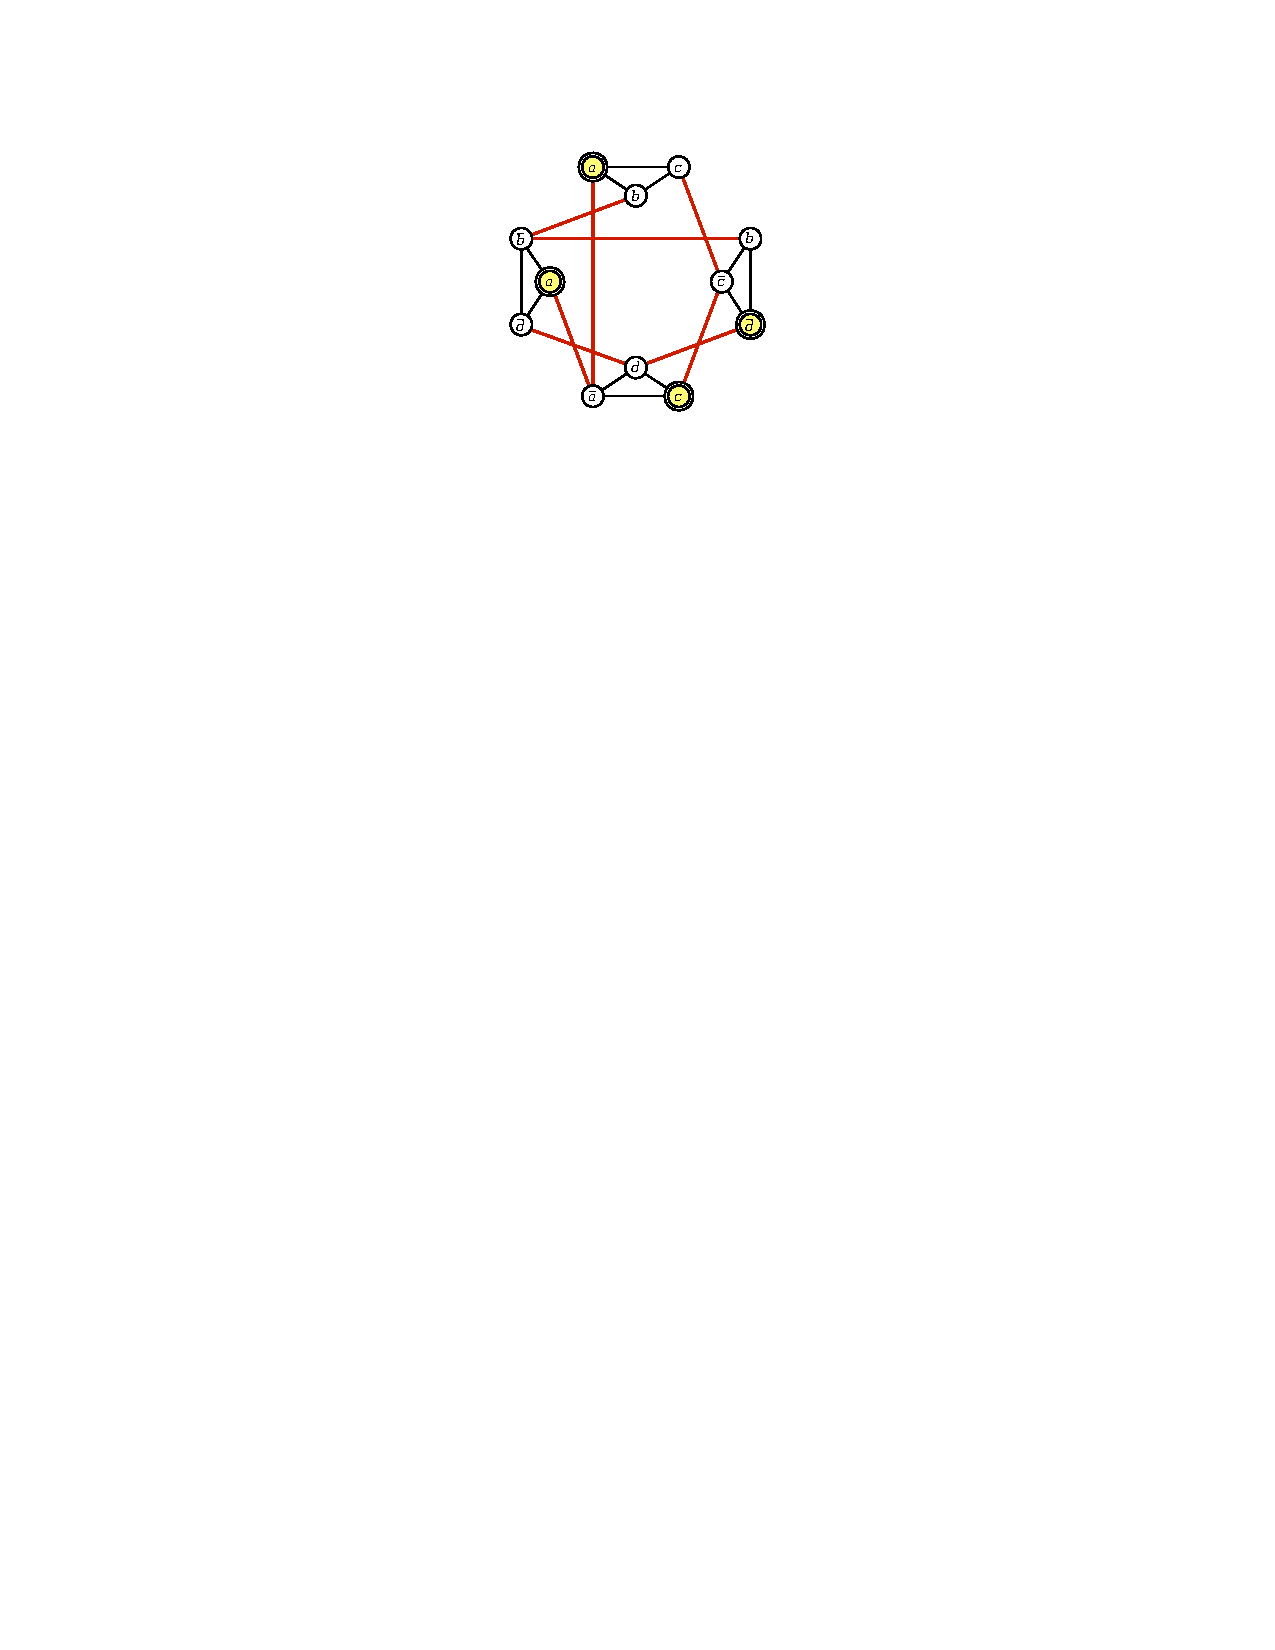
\includegraphics[scale=1.5]{fig/indepset}
    \caption{A graph derived from a 3CNF, and an independent set of size 4}
    \label{fig:indepset}
\end{figure}

The formula is satisfiable if and only if independent set of size $x$:
\begin{itemize}[leftmargin=.75in]
    \item[$\Longrightarrow$] To get satisfying assignment, set each literal from
        independent set to be true.\\
        Since contradictory literals connected by edge, this assignment consistent.\\
        The formula is evaluated to be true since each clause satisfied.
    \item[$\Longleftarrow$] If there is a satisfying assignment, choose one literal for
        each clause that is true.\\
        These literal are independent set in graph since from different clauses and consistent.
\end{itemize}

This proves \textsc{IndepSet}(G,K) is NP-hard.

Since given a subset, can easily check if it is independent set and size $\geq k$,
\textsc{IndepSet}(G,K) $\in$ NP.

Hence, \textsc{IndepSet} in NP-complete.
\end{proof}

\subsection{Clique}
A clique is a subset of vertices where every pair connected.
MaxClique asks for size of largest clique.

\textsc{Clique} is NPC.

Define complement graph $\overline{G}$ as a vertex set, where edge is in $\overline{G}$ if and only if
the edge is not in $G$.
A set if vertices is independent set of $G$ if and only if the same set of vertices is clique in $\overline{G}$.

\subsection{Vertex Cover}
A vertex cover is a set of vertices such that every edge in $G$ is adjacent to vertex in set.
Minimum vertex cover asks for size of smallest vertex cover.
\textsc{VertexCover} asks if vertex cover of size $\leq k$.

\begin{claim}
    A set $I \subseteq V$ is independent set if and only if $V \setminus I$ is the vertex cover.
\end{claim}

\begin{itemize}[leftmargin=.75in]
    \item[$\Longrightarrow$] Consider edge $uv$, cannot have both $u$ and $v \in I$,
        so at least one endpoint in $V \setminus I$.
    \item[$\Longleftarrow$] If $i$ is not independent set, then for some edge $uv$,
        $u,v \in I$, hence $uv$ not covered in $V \setminus I$, (not vertex cover).
\end{itemize}

Hence, \textsc{IndepSet} of size $\geq k$ if and only if vertex cover of size $\leq n-k$.
$I_{max}$ independent set if and only $V \setminus I$ is minimum vertex cover.

\subsection{Some Intuition}
The reduction tree of the problems discussed in the note and homework is shown in \cref{fig:redtree}.

\begin{figure}[H]
    \caption{Reduction Tree}\label{fig:redtree}
    \centering
    \begin{tikzpicture}[every tree node/.style={draw=none},level distance = 1.5cm]
        \Tree [.\textsc{CircuitSAT}
            [.SAT ]
            [.3SAT
                [.\textsc{IndepSet}
                    [.\textsc{Clique} ]
                    [.\textsc{VertexCover}
                        [.\textsc{HittingSet} ]
                    ]
                ]
            ]
        ]
    \end{tikzpicture}
\end{figure}

Here are some other NPC problems:
\begin{itemize}
    \item 3 Coloring
    \item Hamiltonian Path/Cycle
    \item If weighted, TS
\end{itemize}

And here are some Polynomial time problem:
\begin{itemize}
    \item Edge Cover
    \item 2SAT
    \item 2 Coloring
    \item Euler tour in connected even degree vertex graph.
\end{itemize}

And here is the end of the lecture note.


\end{document}
